\documentclass[twoside]{book}

% Packages required by doxygen
\usepackage{fixltx2e}
\usepackage{calc}
\usepackage{doxygen}
\usepackage[export]{adjustbox} % also loads graphicx
\usepackage{graphicx}
\usepackage[utf8]{inputenc}
\usepackage{makeidx}
\usepackage{multicol}
\usepackage{multirow}
\PassOptionsToPackage{warn}{textcomp}
\usepackage{textcomp}
\usepackage[nointegrals]{wasysym}
\usepackage[table]{xcolor}

% Font selection
\usepackage[T1]{fontenc}
\usepackage[scaled=.90]{helvet}
\usepackage{courier}
\usepackage{amssymb}
\usepackage{sectsty}
\renewcommand{\familydefault}{\sfdefault}
\allsectionsfont{%
  \fontseries{bc}\selectfont%
  \color{darkgray}%
}
\renewcommand{\DoxyLabelFont}{%
  \fontseries{bc}\selectfont%
  \color{darkgray}%
}
\newcommand{\+}{\discretionary{\mbox{\scriptsize$\hookleftarrow$}}{}{}}

% Page & text layout
\usepackage{geometry}
\geometry{%
  a4paper,%
  top=2.5cm,%
  bottom=2.5cm,%
  left=2.5cm,%
  right=2.5cm%
}
\tolerance=750
\hfuzz=15pt
\hbadness=750
\setlength{\emergencystretch}{15pt}
\setlength{\parindent}{0cm}
\setlength{\parskip}{3ex plus 2ex minus 2ex}
\makeatletter
\renewcommand{\paragraph}{%
  \@startsection{paragraph}{4}{0ex}{-1.0ex}{1.0ex}{%
    \normalfont\normalsize\bfseries\SS@parafont%
  }%
}
\renewcommand{\subparagraph}{%
  \@startsection{subparagraph}{5}{0ex}{-1.0ex}{1.0ex}{%
    \normalfont\normalsize\bfseries\SS@subparafont%
  }%
}
\makeatother

% Headers & footers
\usepackage{fancyhdr}
\pagestyle{fancyplain}
\fancyhead[LE]{\fancyplain{}{\bfseries\thepage}}
\fancyhead[CE]{\fancyplain{}{}}
\fancyhead[RE]{\fancyplain{}{\bfseries\leftmark}}
\fancyhead[LO]{\fancyplain{}{\bfseries\rightmark}}
\fancyhead[CO]{\fancyplain{}{}}
\fancyhead[RO]{\fancyplain{}{\bfseries\thepage}}
\fancyfoot[LE]{\fancyplain{}{}}
\fancyfoot[CE]{\fancyplain{}{}}
\fancyfoot[RE]{\fancyplain{}{\bfseries\scriptsize Generated by Doxygen }}
\fancyfoot[LO]{\fancyplain{}{\bfseries\scriptsize Generated by Doxygen }}
\fancyfoot[CO]{\fancyplain{}{}}
\fancyfoot[RO]{\fancyplain{}{}}
\renewcommand{\footrulewidth}{0.4pt}
\renewcommand{\chaptermark}[1]{%
  \markboth{#1}{}%
}
\renewcommand{\sectionmark}[1]{%
  \markright{\thesection\ #1}%
}

% Indices & bibliography
\usepackage{natbib}
\usepackage[titles]{tocloft}
\setcounter{tocdepth}{3}
\setcounter{secnumdepth}{5}
\makeindex

% Hyperlinks (required, but should be loaded last)
\usepackage{ifpdf}
\ifpdf
  \usepackage[pdftex,pagebackref=true]{hyperref}
\else
  \usepackage[ps2pdf,pagebackref=true]{hyperref}
\fi
\hypersetup{%
  colorlinks=true,%
  linkcolor=blue,%
  citecolor=blue,%
  unicode%
}

% Custom commands
\newcommand{\clearemptydoublepage}{%
  \newpage{\pagestyle{empty}\cleardoublepage}%
}

\usepackage{caption}
\captionsetup{labelsep=space,justification=centering,font={bf},singlelinecheck=off,skip=4pt,position=top}

%===== C O N T E N T S =====

\begin{document}

% Titlepage & ToC
\hypersetup{pageanchor=false,
             bookmarksnumbered=true,
             pdfencoding=unicode
            }
\pagenumbering{roman}
\begin{titlepage}
\vspace*{7cm}
\begin{center}%
{\Large Supermarket Cleaning Robot }\\
\vspace*{1cm}
{\large Generated by Doxygen 1.8.11}\\
\end{center}
\end{titlepage}
\clearemptydoublepage
\tableofcontents
\clearemptydoublepage
\pagenumbering{arabic}
\hypersetup{pageanchor=true}

%--- Begin generated contents ---
\chapter{Project X}
\label{md_README}
\hypertarget{md_README}{}
\href{https://travis-ci.org/urastogi885/Supermarket-Cleaning-Robot}{\tt } \href{https://coveralls.io/github/urastogi885/Supermarket-Cleaning-Robot?branch=master}{\tt } \subsection*{\href{https://github.com/urastogi885/Supermarket-Cleaning-Robot/blob/master/LICENSE}{\tt } }

\subsection*{Overview}

According to a study done in Morrisville, North Carolina, the Walmart Supercenter located in the town receives about 10,000 people per day. Unquestionably, the actual foot traffic depends on a variety of factors, but we cannot disregard that supermarkets are one of the busiest places in a town. The more the number of people, the more likely it is for the store to become dirty. It always begets frustration among workers to maintain the store at its most pristine level. Our supermarket cleaning robot can remove the stress of cleanliness by performing the tasks of an employee.

Currently, most of the robots are only capable of executing a single task. It turns out to be expensive for a store owner to buy a robot that can perform a single task. We propose to develop a robot that can perform various maintenance tasks. The robot will be able to maintain cleanliness as well as make supermarkets autonomous. The robot will able to clean aisles, stack up empty rows, and collect fallen items.

For prototyping, we are focusing on only one task that is identifying and collecting the items using the robot. The robot will roam in a supermarket like environment in Gazebo and identify the type of items that it needs to collect. It identifies the item using a camera, mounted on its base, and moves towards the fallen item. Here, we are considering objects such as food, soft drinks cans and it is assumed that the robot will already know the type of item that it needs to pick. As the robot reaches the location of the item and touches it, the item will vanish depicting that the item is collected using a suction cup. The robot will traverse randomly in the supermarket and keep on collecting a can. We are focusing on the detection of cans using the Open\+CV to improve the processing of the detection feature. In addition to this, the robot has an obstacle avoidance feature that is used to prevent the robot from colliding from obstacles such as humans, uninteresting items and walls/shelves.

 {\bfseries Figure 1 -\/ Robot approaching towards the cans lying on the ground to collect them} 

\subsection*{Team Members}


\begin{DoxyItemize}
\item \href{https://github.com/urastogi885}{\tt Umang Rastogi} -\/ Pursuing masters in Robotics at University of Maryland $\vert$ B.\+Tech in Electronics \& Communication Engineering
\item \href{https://github.com/namangupta98}{\tt Naman Gupta} -\/ Grad Student at University of Maryland, pursuing M.\+Eng. in Robotics.
\end{DoxyItemize}

\subsection*{A\+IP and Sprint Documents}


\begin{DoxyItemize}
\item Click on this \href{https://docs.google.com/spreadsheets/d/1k6e7rM7TTvE5w2fQ_wuSDY_giNWaVuCHeImB6D53lT4/edit?usp=sharing}{\tt {\itshape link}} to access our A\+IP Google Sheet.
\item Click on this \href{https://docs.google.com/document/d/1iQZUstgoCCvtSvlcv1_xpxGW6ntUbkOpcgMuvrSP_ms/edit?usp=sharing}{\tt {\itshape link}} to access our Sprint notes document.
\end{DoxyItemize}

\subsection*{Accessing the U\+ML Diagrams}


\begin{DoxyItemize}
\item Open the {\itshape U\+ML} directory of the project.
\item Access U\+ML diagrams from the {\itshape initial} folder located within {\itshape U\+ML} sub-\/directory.
\end{DoxyItemize}

\subsection*{A\+PI Documentations}


\begin{DoxyItemize}
\item \href{http://gazebosim.org/tutorials?tut=model_population&cat=build_world}{\tt Gazebo Population Tag}
\item \href{http://wiki.ros.org/cv_bridge/Tutorials/UsingCvBridgeToConvertBetweenROSImagesAndOpenCVImages}{\tt cv\+\_\+bridge}
\item \href{https://docs.opencv.org/master/de/da9/tutorial_template_matching.html}{\tt Template Matching}
\end{DoxyItemize}

\subsection*{Dependencies}


\begin{DoxyItemize}
\item Ubuntu 16.\+04
\item R\+OS Kinetic
\item Gazebo
\item \hyperlink{classTurtlebot}{Turtlebot} Packages
\end{DoxyItemize}

\subsection*{Install Dependences}


\begin{DoxyItemize}
\item This project was developed using R\+OS Kinetic.
\item It is highly recommended that R\+OS Kinetic is properly installed on your system before the use of this project.
\item Follow the instructions on the \href{http://wiki.ros.org/kinetic/Installation/Ubuntu}{\tt {\itshape R\+OS kinetic install tutorial page}} to install $\ast$$\ast$$\ast$\+Full-\/\+Desktop Version$\ast$$\ast$$\ast$ of R\+OS Kinetic.
\item The full-\/version would help you install {\itshape Gazebo} as well. If you have R\+OS Kinetic pre-\/installed on your machine, use the following \href{http://gazebosim.org/tutorials?tut=install_ubuntu&cat=install}{\tt {\itshape link}} to just install {\itshape Gazebo} on your machine.
\item Ensure successful installation by running {\itshape Gazebo} via your terminal window\+: 
\begin{DoxyCode}
1 gazebo
\end{DoxyCode}

\item An empty window of {\itshape Gazebo Simulator} should be launched.
\item Make sure that turtlebot packages have been installed on your machine using the following commands\+: 
\begin{DoxyCode}
1 roslaunch turtlebot\_gazebo turtlebot\_world.launch
\end{DoxyCode}

\item A window of {\itshape Gazebo Simulator} with various items and a turtlebot should be launched.
\item If an error pops up upo launching the turtlebot world, then install the necessary turtlebot packages\+: 
\begin{DoxyCode}
1 sudo apt install ros-kinetic-turtlebot-gazebo ros-kinetic-turtlebot-apps
       ros-kinetic-turtlebot-rviz-launchers
\end{DoxyCode}

\item Create your R\+OS workspace by following instructions on the \href{http://wiki.ros.org/catkin/Tutorials/create_a_workspace}{\tt {\itshape create R\+OS workspace tutortial page}}.
\end{DoxyItemize}

\subsection*{Known Bugs and Issues}

This project is under-\/development. Currently, we are facing build issues. Sorry for the inconvenience.

\subsection*{Build}


\begin{DoxyItemize}
\item $\ast$$\ast$$\ast$\+Ignore this section$\ast$$\ast$$\ast$ as nothing to be built has been added yet.
\item Even if you run the following, it will not impact your existing workspace.
\item Switch to your {\itshape src} sub-\/directory of your R\+OS workspace to clone this repository. 
\begin{DoxyCode}
1 <ROS Workspace>/src
\end{DoxyCode}

\item Run the following commands to clone and build this project\+: 
\begin{DoxyCode}
1 git clone --recursive https://github.com/urastogi885/obstacle\_avoidance\_simulation
2 git checkout Phase3
3 cd ..
4 catkin\_make
\end{DoxyCode}

\end{DoxyItemize}

\subsection*{Test}

Close and terminate everything including rosmaster. In a new terminal, switch to the R\+OS workspace and build the tests. Type


\begin{DoxyCode}
1 cd catkin\_ws
2 source devel/setup.bash
3 catkin\_make run\_tests\_test\_project\_x\_robot
\end{DoxyCode}


\subsection*{Run}

Now, we use launch file to run. In a new terminal, type


\begin{DoxyCode}
1 cd catkin\_ws
2 source devel/setup.bash
3 roslaunch supermarket\_cleaning\_robot object\_collection.launch
\end{DoxyCode}


\subsection*{Doxygen}

To install doxygen run the following command\+:


\begin{DoxyCode}
1 sudo apt-get install doxygen
\end{DoxyCode}
 Now from the cloned directory run\+:


\begin{DoxyCode}
1 doxygen doxygen
\end{DoxyCode}


Generated doxygen files are in html format and you can find them in ./docs folder. With the following command


\begin{DoxyCode}
1 firefox docs/html/index.html
\end{DoxyCode}


\subsection*{Demo}

We will update in the next phase by next week. 
\chapter{Class Index}
\section{Class List}
Here are the classes, structs, unions and interfaces with brief descriptions\+:\begin{DoxyCompactList}
\item\contentsline{section}{\hyperlink{classObjectDectection}{Object\+Dectection} }{\pageref{classObjectDectection}}{}
\item\contentsline{section}{\hyperlink{classObstacleAvoidance}{Obstacle\+Avoidance} }{\pageref{classObstacleAvoidance}}{}
\item\contentsline{section}{\hyperlink{classTurtlebot}{Turtlebot} \\*Add R\+OS headers }{\pageref{classTurtlebot}}{}
\end{DoxyCompactList}

\chapter{File Index}
\section{File List}
Here is a list of all files with brief descriptions\+:\begin{DoxyCompactList}
\item\contentsline{section}{include/object\+\_\+detection/\hyperlink{object__detection_8h}{object\+\_\+detection.\+h} \\*Library header file to implement object detection  Deploys template matching to detect object in the bot\textquotesingle{}s world }{\pageref{object__detection_8h}}{}
\item\contentsline{section}{include/obstacle\+\_\+avoidance/\hyperlink{obstacle__avoidance_8h}{obstacle\+\_\+avoidance.\+h} \\*Library header file to implement obstacle avoidance }{\pageref{obstacle__avoidance_8h}}{}
\item\contentsline{section}{include/turtlebot/\hyperlink{turtlebot_8h}{turtlebot.\+h} \\*Library header file to control motion of the bot  Takes input from both, obstacle avoidance and object detection }{\pageref{turtlebot_8h}}{}
\item\contentsline{section}{src/\hyperlink{obstacle__avoidance_8cpp}{obstacle\+\_\+avoidance.\+cpp} }{\pageref{obstacle__avoidance_8cpp}}{}
\item\contentsline{section}{src/\hyperlink{turtlebot_8cpp}{turtlebot.\+cpp} \\*Source file to implement turtlebot class  Controls the motion of the bot using obstacle avoidance and go-\/to-\/goal strategies }{\pageref{turtlebot_8cpp}}{}
\item\contentsline{section}{test/\hyperlink{main_8cpp}{main.\+cpp} \\*Test implementation of class test }{\pageref{main_8cpp}}{}
\item\contentsline{section}{test/\hyperlink{obstacle__avoidance__test_8cpp}{obstacle\+\_\+avoidance\+\_\+test.\+cpp} \\*Class test implementation of class \hyperlink{classObstacleAvoidance}{Obstacle\+Avoidance} }{\pageref{obstacle__avoidance__test_8cpp}}{}
\item\contentsline{section}{test/\hyperlink{turtlebot__test_8cpp}{turtlebot\+\_\+test.\+cpp} }{\pageref{turtlebot__test_8cpp}}{}
\end{DoxyCompactList}

\chapter{Class Documentation}
\hypertarget{classObjectDetection}{}\section{Object\+Detection Class Reference}
\label{classObjectDetection}\index{Object\+Detection@{Object\+Detection}}


{\ttfamily \#include $<$object\+\_\+detection.\+h$>$}

\subsection*{Public Member Functions}
\begin{DoxyCompactItemize}
\item 
\hyperlink{classObjectDetection_a6ccb25952ecc45811451c5cb623e23ee}{Object\+Detection} ()
\begin{DoxyCompactList}\small\item\em Constructor for object detection class. \end{DoxyCompactList}\item 
\hyperlink{classObjectDetection_ad5d9d344ab55095927725733590f0da5}{$\sim$\+Object\+Detection} ()
\begin{DoxyCompactList}\small\item\em Destructor for object detection class. \end{DoxyCompactList}\item 
void \hyperlink{classObjectDetection_abb6ea33423e081c37bd38e55f1347f52}{convert\+Image} (const sensor\+\_\+msgs\+::\+Image\+::\+Const\+Ptr \&image\+Data)
\begin{DoxyCompactList}\small\item\em Callback function for image data. \end{DoxyCompactList}\item 
bool \hyperlink{classObjectDetection_a63d13b70232d3d076a6c543c03f9c9ff}{detect\+Object} (cv\+::\+Mat image)
\begin{DoxyCompactList}\small\item\em Method to detect object using hsv. \end{DoxyCompactList}\item 
cv\+::\+Mat \hyperlink{classObjectDetection_a0f559ec8747dca4882aa3fe8f21e0fb8}{apply\+Gauss\+Blur} (cv\+::\+Mat cvt\+Image)
\begin{DoxyCompactList}\small\item\em Method to convert gaussian filter on the image. \end{DoxyCompactList}\item 
cv\+::\+Rect \hyperlink{classObjectDetection_a897f179535427f66bc9f849b1daff904}{get\+Object\+Boundary} () const 
\begin{DoxyCompactList}\small\item\em Get boundary of the object in the image. \end{DoxyCompactList}\item 
void \hyperlink{classObjectDetection_af3c1adc86fa3950f0325e5c6de7c9a2e}{set\+Object\+Boundary} (cv\+::\+Rect bounding\+Box)
\begin{DoxyCompactList}\small\item\em Set object boundary. \end{DoxyCompactList}\item 
bool \hyperlink{classObjectDetection_ac1e795be46de92c3e7c2f050d805d601}{get\+Object\+Detected} () const 
\begin{DoxyCompactList}\small\item\em Get object detected. \end{DoxyCompactList}\item 
void \hyperlink{classObjectDetection_a1f0c0d87bb3fdc9082c8f4c450bbf1fb}{set\+Object\+Detected} (bool object)
\begin{DoxyCompactList}\small\item\em Set object detected. \end{DoxyCompactList}\end{DoxyCompactItemize}
\subsection*{Public Attributes}
\begin{DoxyCompactItemize}
\item 
cv\+::\+Mat \hyperlink{classObjectDetection_ab3a61dd408dd36da96f7398f14a1a054}{converted\+Image}
\begin{DoxyCompactList}\small\item\em Container to store converted image from cv\+\_\+bridge. \end{DoxyCompactList}\end{DoxyCompactItemize}


\subsection{Constructor \& Destructor Documentation}
\index{Object\+Detection@{Object\+Detection}!Object\+Detection@{Object\+Detection}}
\index{Object\+Detection@{Object\+Detection}!Object\+Detection@{Object\+Detection}}
\subsubsection[{\texorpdfstring{Object\+Detection()}{ObjectDetection()}}]{\setlength{\rightskip}{0pt plus 5cm}Object\+Detection\+::\+Object\+Detection (
\begin{DoxyParamCaption}
{}
\end{DoxyParamCaption}
)}\hypertarget{classObjectDetection_a6ccb25952ecc45811451c5cb623e23ee}{}\label{classObjectDetection_a6ccb25952ecc45811451c5cb623e23ee}


Constructor for object detection class. 


\begin{DoxyParams}{Parameters}
{\em none} & \\
\hline
\end{DoxyParams}
\begin{DoxyReturn}{Returns}
none 
\end{DoxyReturn}
Subscribe to turtlebot camera to get feed from the camera \index{Object\+Detection@{Object\+Detection}!````~Object\+Detection@{$\sim$\+Object\+Detection}}
\index{````~Object\+Detection@{$\sim$\+Object\+Detection}!Object\+Detection@{Object\+Detection}}
\subsubsection[{\texorpdfstring{$\sim$\+Object\+Detection()}{~ObjectDetection()}}]{\setlength{\rightskip}{0pt plus 5cm}Object\+Detection\+::$\sim$\+Object\+Detection (
\begin{DoxyParamCaption}
{}
\end{DoxyParamCaption}
)}\hypertarget{classObjectDetection_ad5d9d344ab55095927725733590f0da5}{}\label{classObjectDetection_ad5d9d344ab55095927725733590f0da5}


Destructor for object detection class. 


\begin{DoxyParams}{Parameters}
{\em none} & \\
\hline
\end{DoxyParams}
\begin{DoxyReturn}{Returns}
none 
\end{DoxyReturn}


\subsection{Member Function Documentation}
\index{Object\+Detection@{Object\+Detection}!apply\+Gauss\+Blur@{apply\+Gauss\+Blur}}
\index{apply\+Gauss\+Blur@{apply\+Gauss\+Blur}!Object\+Detection@{Object\+Detection}}
\subsubsection[{\texorpdfstring{apply\+Gauss\+Blur(cv\+::\+Mat cvt\+Image)}{applyGaussBlur(cv::Mat cvtImage)}}]{\setlength{\rightskip}{0pt plus 5cm}cv\+::\+Mat Object\+Detection\+::apply\+Gauss\+Blur (
\begin{DoxyParamCaption}
\item[{cv\+::\+Mat}]{cvt\+Image}
\end{DoxyParamCaption}
)}\hypertarget{classObjectDetection_a0f559ec8747dca4882aa3fe8f21e0fb8}{}\label{classObjectDetection_a0f559ec8747dca4882aa3fe8f21e0fb8}


Method to convert gaussian filter on the image. 


\begin{DoxyParams}{Parameters}
{\em Converted} & opencv image of type cv\+::\+Mat \\
\hline
\end{DoxyParams}
\begin{DoxyReturn}{Returns}
Image blurred using gaussian filter of type cv\+::\+Mat 
\end{DoxyReturn}
Apply gaussian filter \index{Object\+Detection@{Object\+Detection}!convert\+Image@{convert\+Image}}
\index{convert\+Image@{convert\+Image}!Object\+Detection@{Object\+Detection}}
\subsubsection[{\texorpdfstring{convert\+Image(const sensor\+\_\+msgs\+::\+Image\+::\+Const\+Ptr \&image\+Data)}{convertImage(const sensor_msgs::Image::ConstPtr &imageData)}}]{\setlength{\rightskip}{0pt plus 5cm}void Object\+Detection\+::convert\+Image (
\begin{DoxyParamCaption}
\item[{const sensor\+\_\+msgs\+::\+Image\+::\+Const\+Ptr \&}]{image\+Data}
\end{DoxyParamCaption}
)}\hypertarget{classObjectDetection_abb6ea33423e081c37bd38e55f1347f52}{}\label{classObjectDetection_abb6ea33423e081c37bd38e55f1347f52}


Callback function for image data. 


\begin{DoxyParams}{Parameters}
{\em Image} & data from camera node \\
\hline
\end{DoxyParams}
\begin{DoxyReturn}{Returns}
none  Convert R\+OS image message to CV image 
\end{DoxyReturn}
Create an object cv\+\_\+ptr that bridges the R\+OS image and Open\+CV image

Wait for 30ms \index{Object\+Detection@{Object\+Detection}!detect\+Object@{detect\+Object}}
\index{detect\+Object@{detect\+Object}!Object\+Detection@{Object\+Detection}}
\subsubsection[{\texorpdfstring{detect\+Object(cv\+::\+Mat image)}{detectObject(cv::Mat image)}}]{\setlength{\rightskip}{0pt plus 5cm}bool Object\+Detection\+::detect\+Object (
\begin{DoxyParamCaption}
\item[{cv\+::\+Mat}]{image}
\end{DoxyParamCaption}
)}\hypertarget{classObjectDetection_a63d13b70232d3d076a6c543c03f9c9ff}{}\label{classObjectDetection_a63d13b70232d3d076a6c543c03f9c9ff}


Method to detect object using hsv. 


\begin{DoxyParams}{Parameters}
{\em Image} & gaussian filtered image of type cv\+::\+Mat \\
\hline
\end{DoxyParams}
\begin{DoxyReturn}{Returns}
Match found of type bool 
\end{DoxyReturn}
Image conversion from B\+GR to H\+SV

Detect hsv within the set limits

Get image size to modify size of mask image

Find contours for better visualization

Check if contours exist in the image

Find contour with maximum area

Set boundary of the object in the image

Draw the rectangle using the bounding box

Mask image to limit the future turns affecting the output \index{Object\+Detection@{Object\+Detection}!get\+Object\+Boundary@{get\+Object\+Boundary}}
\index{get\+Object\+Boundary@{get\+Object\+Boundary}!Object\+Detection@{Object\+Detection}}
\subsubsection[{\texorpdfstring{get\+Object\+Boundary() const }{getObjectBoundary() const }}]{\setlength{\rightskip}{0pt plus 5cm}cv\+::\+Rect Object\+Detection\+::get\+Object\+Boundary (
\begin{DoxyParamCaption}
{}
\end{DoxyParamCaption}
) const\hspace{0.3cm}{\ttfamily [inline]}}\hypertarget{classObjectDetection_a897f179535427f66bc9f849b1daff904}{}\label{classObjectDetection_a897f179535427f66bc9f849b1daff904}


Get boundary of the object in the image. 


\begin{DoxyParams}{Parameters}
{\em none} & \\
\hline
\end{DoxyParams}
\begin{DoxyReturn}{Returns}
rectangular box containing the object 
\end{DoxyReturn}
\index{Object\+Detection@{Object\+Detection}!get\+Object\+Detected@{get\+Object\+Detected}}
\index{get\+Object\+Detected@{get\+Object\+Detected}!Object\+Detection@{Object\+Detection}}
\subsubsection[{\texorpdfstring{get\+Object\+Detected() const }{getObjectDetected() const }}]{\setlength{\rightskip}{0pt plus 5cm}bool Object\+Detection\+::get\+Object\+Detected (
\begin{DoxyParamCaption}
{}
\end{DoxyParamCaption}
) const\hspace{0.3cm}{\ttfamily [inline]}}\hypertarget{classObjectDetection_ac1e795be46de92c3e7c2f050d805d601}{}\label{classObjectDetection_ac1e795be46de92c3e7c2f050d805d601}


Get object detected. 


\begin{DoxyParams}{Parameters}
{\em none} & \\
\hline
\end{DoxyParams}
\begin{DoxyReturn}{Returns}
Object detected or not of type bool 
\end{DoxyReturn}
\index{Object\+Detection@{Object\+Detection}!set\+Object\+Boundary@{set\+Object\+Boundary}}
\index{set\+Object\+Boundary@{set\+Object\+Boundary}!Object\+Detection@{Object\+Detection}}
\subsubsection[{\texorpdfstring{set\+Object\+Boundary(cv\+::\+Rect bounding\+Box)}{setObjectBoundary(cv::Rect boundingBox)}}]{\setlength{\rightskip}{0pt plus 5cm}void Object\+Detection\+::set\+Object\+Boundary (
\begin{DoxyParamCaption}
\item[{cv\+::\+Rect}]{bounding\+Box}
\end{DoxyParamCaption}
)\hspace{0.3cm}{\ttfamily [inline]}}\hypertarget{classObjectDetection_af3c1adc86fa3950f0325e5c6de7c9a2e}{}\label{classObjectDetection_af3c1adc86fa3950f0325e5c6de7c9a2e}


Set object boundary. 


\begin{DoxyParams}{Parameters}
{\em Bounding\+Box} & reactagular boundary of the object \\
\hline
\end{DoxyParams}
\begin{DoxyReturn}{Returns}
none 
\end{DoxyReturn}
\index{Object\+Detection@{Object\+Detection}!set\+Object\+Detected@{set\+Object\+Detected}}
\index{set\+Object\+Detected@{set\+Object\+Detected}!Object\+Detection@{Object\+Detection}}
\subsubsection[{\texorpdfstring{set\+Object\+Detected(bool object)}{setObjectDetected(bool object)}}]{\setlength{\rightskip}{0pt plus 5cm}void Object\+Detection\+::set\+Object\+Detected (
\begin{DoxyParamCaption}
\item[{bool}]{object}
\end{DoxyParamCaption}
)\hspace{0.3cm}{\ttfamily [inline]}}\hypertarget{classObjectDetection_a1f0c0d87bb3fdc9082c8f4c450bbf1fb}{}\label{classObjectDetection_a1f0c0d87bb3fdc9082c8f4c450bbf1fb}


Set object detected. 


\begin{DoxyParams}{Parameters}
{\em Object} & detected status \\
\hline
\end{DoxyParams}
\begin{DoxyReturn}{Returns}
none 
\end{DoxyReturn}


\subsection{Member Data Documentation}
\index{Object\+Detection@{Object\+Detection}!converted\+Image@{converted\+Image}}
\index{converted\+Image@{converted\+Image}!Object\+Detection@{Object\+Detection}}
\subsubsection[{\texorpdfstring{converted\+Image}{convertedImage}}]{\setlength{\rightskip}{0pt plus 5cm}cv\+::\+Mat Object\+Detection\+::converted\+Image}\hypertarget{classObjectDetection_ab3a61dd408dd36da96f7398f14a1a054}{}\label{classObjectDetection_ab3a61dd408dd36da96f7398f14a1a054}


Container to store converted image from cv\+\_\+bridge. 



The documentation for this class was generated from the following files\+:\begin{DoxyCompactItemize}
\item 
include/object\+\_\+detection/\hyperlink{object__detection_8h}{object\+\_\+detection.\+h}\item 
src/\hyperlink{object__detection_8cpp}{object\+\_\+detection.\+cpp}\end{DoxyCompactItemize}

\hypertarget{classObstacleAvoidance}{}\section{Obstacle\+Avoidance Class Reference}
\label{classObstacleAvoidance}\index{Obstacle\+Avoidance@{Obstacle\+Avoidance}}


{\ttfamily \#include $<$obstacle\+\_\+avoidance.\+h$>$}

\subsection*{Public Member Functions}
\begin{DoxyCompactItemize}
\item 
\hyperlink{classObstacleAvoidance_adff25e3149ac860f48af277913c6e51e}{Obstacle\+Avoidance} ()
\begin{DoxyCompactList}\small\item\em Constructor for obstacle avoidance class. \end{DoxyCompactList}\item 
\hyperlink{classObstacleAvoidance_acc575828426b0c1f499f0d2de8e8adc9}{Obstacle\+Avoidance} (float dist\+Threshold)
\begin{DoxyCompactList}\small\item\em Constructor for obstacle avoidance class. \end{DoxyCompactList}\item 
\hyperlink{classObstacleAvoidance_aead959d605cc5599afde7da5e66b24f7}{$\sim$\+Obstacle\+Avoidance} ()
\begin{DoxyCompactList}\small\item\em Destructor for obstacle avoidance class. \end{DoxyCompactList}\item 
void \hyperlink{classObstacleAvoidance_af03480261c682c2b9b4026f377cc9e3f}{laser\+Sensor\+Callback} (const sensor\+\_\+msgs\+::\+Laser\+Scan\+::\+Const\+Ptr \&sensor\+Data)
\begin{DoxyCompactList}\small\item\em Callback function for subscriber. \end{DoxyCompactList}\item 
bool \hyperlink{classObstacleAvoidance_a10de6174bbf71748bb9467981c6f9ab4}{check\+Obstacle} ()
\begin{DoxyCompactList}\small\item\em Checks if obstacle is present within safe distance. \end{DoxyCompactList}\item 
bool \hyperlink{classObstacleAvoidance_a9bc10665f077a2a22c203289e187ebb3}{get\+Obstacle\+Detected} () const 
\begin{DoxyCompactList}\small\item\em get obstacle detected \end{DoxyCompactList}\item 
void \hyperlink{classObstacleAvoidance_ab905f3e115e16482e7f8a6b24e0f3cf1}{set\+Obstacle\+Detected} (bool obstacle)
\begin{DoxyCompactList}\small\item\em set obstacle detected \end{DoxyCompactList}\end{DoxyCompactItemize}


\subsection{Constructor \& Destructor Documentation}
\index{Obstacle\+Avoidance@{Obstacle\+Avoidance}!Obstacle\+Avoidance@{Obstacle\+Avoidance}}
\index{Obstacle\+Avoidance@{Obstacle\+Avoidance}!Obstacle\+Avoidance@{Obstacle\+Avoidance}}
\subsubsection[{\texorpdfstring{Obstacle\+Avoidance()}{ObstacleAvoidance()}}]{\setlength{\rightskip}{0pt plus 5cm}Obstacle\+Avoidance\+::\+Obstacle\+Avoidance (
\begin{DoxyParamCaption}
{}
\end{DoxyParamCaption}
)}\hypertarget{classObstacleAvoidance_adff25e3149ac860f48af277913c6e51e}{}\label{classObstacleAvoidance_adff25e3149ac860f48af277913c6e51e}


Constructor for obstacle avoidance class. 


\begin{DoxyParams}{Parameters}
{\em none} & \\
\hline
\end{DoxyParams}
\begin{DoxyReturn}{Returns}
a constructor has no return 
\end{DoxyReturn}
Initialize the current value of velocities in m/s and rad/s

Initialize obstacle detected value with false

Initialize safe distance from an obstacle in meters

Subscribe for data from the laser sensor on the scan topic \index{Obstacle\+Avoidance@{Obstacle\+Avoidance}!Obstacle\+Avoidance@{Obstacle\+Avoidance}}
\index{Obstacle\+Avoidance@{Obstacle\+Avoidance}!Obstacle\+Avoidance@{Obstacle\+Avoidance}}
\subsubsection[{\texorpdfstring{Obstacle\+Avoidance(float dist\+Threshold)}{ObstacleAvoidance(float distThreshold)}}]{\setlength{\rightskip}{0pt plus 5cm}Obstacle\+Avoidance\+::\+Obstacle\+Avoidance (
\begin{DoxyParamCaption}
\item[{float}]{dist\+Threshold}
\end{DoxyParamCaption}
)\hspace{0.3cm}{\ttfamily [explicit]}}\hypertarget{classObstacleAvoidance_acc575828426b0c1f499f0d2de8e8adc9}{}\label{classObstacleAvoidance_acc575828426b0c1f499f0d2de8e8adc9}


Constructor for obstacle avoidance class. 


\begin{DoxyParams}{Parameters}
{\em safe} & distance from an obstacle \\
\hline
\end{DoxyParams}
\begin{DoxyReturn}{Returns}
a constructor has no return 
\end{DoxyReturn}
Initialize obstacle detected value with false

Initialize safe distance from an obstacle in meters

Subscribe for data from the laser sensor on the scan topic \index{Obstacle\+Avoidance@{Obstacle\+Avoidance}!````~Obstacle\+Avoidance@{$\sim$\+Obstacle\+Avoidance}}
\index{````~Obstacle\+Avoidance@{$\sim$\+Obstacle\+Avoidance}!Obstacle\+Avoidance@{Obstacle\+Avoidance}}
\subsubsection[{\texorpdfstring{$\sim$\+Obstacle\+Avoidance()}{~ObstacleAvoidance()}}]{\setlength{\rightskip}{0pt plus 5cm}Obstacle\+Avoidance\+::$\sim$\+Obstacle\+Avoidance (
\begin{DoxyParamCaption}
{}
\end{DoxyParamCaption}
)}\hypertarget{classObstacleAvoidance_aead959d605cc5599afde7da5e66b24f7}{}\label{classObstacleAvoidance_aead959d605cc5599afde7da5e66b24f7}


Destructor for obstacle avoidance class. 


\begin{DoxyParams}{Parameters}
{\em none} & \\
\hline
\end{DoxyParams}
\begin{DoxyReturn}{Returns}
a destrcutor has no return 
\end{DoxyReturn}


\subsection{Member Function Documentation}
\index{Obstacle\+Avoidance@{Obstacle\+Avoidance}!check\+Obstacle@{check\+Obstacle}}
\index{check\+Obstacle@{check\+Obstacle}!Obstacle\+Avoidance@{Obstacle\+Avoidance}}
\subsubsection[{\texorpdfstring{check\+Obstacle()}{checkObstacle()}}]{\setlength{\rightskip}{0pt plus 5cm}bool Obstacle\+Avoidance\+::check\+Obstacle (
\begin{DoxyParamCaption}
{}
\end{DoxyParamCaption}
)}\hypertarget{classObstacleAvoidance_a10de6174bbf71748bb9467981c6f9ab4}{}\label{classObstacleAvoidance_a10de6174bbf71748bb9467981c6f9ab4}


Checks if obstacle is present within safe distance. 


\begin{DoxyParams}{Parameters}
{\em none} & \\
\hline
\end{DoxyParams}
\begin{DoxyReturn}{Returns}
boolean obstacle found or not 
\end{DoxyReturn}
Check if obstacle is ahead \index{Obstacle\+Avoidance@{Obstacle\+Avoidance}!get\+Obstacle\+Detected@{get\+Obstacle\+Detected}}
\index{get\+Obstacle\+Detected@{get\+Obstacle\+Detected}!Obstacle\+Avoidance@{Obstacle\+Avoidance}}
\subsubsection[{\texorpdfstring{get\+Obstacle\+Detected() const }{getObstacleDetected() const }}]{\setlength{\rightskip}{0pt plus 5cm}bool Obstacle\+Avoidance\+::get\+Obstacle\+Detected (
\begin{DoxyParamCaption}
{}
\end{DoxyParamCaption}
) const\hspace{0.3cm}{\ttfamily [inline]}}\hypertarget{classObstacleAvoidance_a9bc10665f077a2a22c203289e187ebb3}{}\label{classObstacleAvoidance_a9bc10665f077a2a22c203289e187ebb3}


get obstacle detected 


\begin{DoxyParams}{Parameters}
{\em none} & \\
\hline
\end{DoxyParams}
\begin{DoxyReturn}{Returns}
boolean obstacle detected or not 
\end{DoxyReturn}
\index{Obstacle\+Avoidance@{Obstacle\+Avoidance}!laser\+Sensor\+Callback@{laser\+Sensor\+Callback}}
\index{laser\+Sensor\+Callback@{laser\+Sensor\+Callback}!Obstacle\+Avoidance@{Obstacle\+Avoidance}}
\subsubsection[{\texorpdfstring{laser\+Sensor\+Callback(const sensor\+\_\+msgs\+::\+Laser\+Scan\+::\+Const\+Ptr \&sensor\+Data)}{laserSensorCallback(const sensor_msgs::LaserScan::ConstPtr &sensorData)}}]{\setlength{\rightskip}{0pt plus 5cm}void Obstacle\+Avoidance\+::laser\+Sensor\+Callback (
\begin{DoxyParamCaption}
\item[{const sensor\+\_\+msgs\+::\+Laser\+Scan\+::\+Const\+Ptr \&}]{sensor\+Data}
\end{DoxyParamCaption}
)}\hypertarget{classObstacleAvoidance_af03480261c682c2b9b4026f377cc9e3f}{}\label{classObstacleAvoidance_af03480261c682c2b9b4026f377cc9e3f}


Callback function for subscriber. 


\begin{DoxyParams}{Parameters}
{\em messsage} & data from Laser\+Scan node \\
\hline
\end{DoxyParams}
\begin{DoxyReturn}{Returns}
void 
\end{DoxyReturn}
Read sensor data to get obstacle distances with respect to the robot \index{Obstacle\+Avoidance@{Obstacle\+Avoidance}!set\+Obstacle\+Detected@{set\+Obstacle\+Detected}}
\index{set\+Obstacle\+Detected@{set\+Obstacle\+Detected}!Obstacle\+Avoidance@{Obstacle\+Avoidance}}
\subsubsection[{\texorpdfstring{set\+Obstacle\+Detected(bool obstacle)}{setObstacleDetected(bool obstacle)}}]{\setlength{\rightskip}{0pt plus 5cm}void Obstacle\+Avoidance\+::set\+Obstacle\+Detected (
\begin{DoxyParamCaption}
\item[{bool}]{obstacle}
\end{DoxyParamCaption}
)\hspace{0.3cm}{\ttfamily [inline]}}\hypertarget{classObstacleAvoidance_ab905f3e115e16482e7f8a6b24e0f3cf1}{}\label{classObstacleAvoidance_ab905f3e115e16482e7f8a6b24e0f3cf1}


set obstacle detected 


\begin{DoxyParams}{Parameters}
{\em obstacle} & detected status \\
\hline
\end{DoxyParams}
\begin{DoxyReturn}{Returns}
void 
\end{DoxyReturn}


The documentation for this class was generated from the following files\+:\begin{DoxyCompactItemize}
\item 
include/obstacle\+\_\+avoidance/\hyperlink{obstacle__avoidance_8h}{obstacle\+\_\+avoidance.\+h}\item 
src/\hyperlink{obstacle__avoidance_8cpp}{obstacle\+\_\+avoidance.\+cpp}\end{DoxyCompactItemize}

\hypertarget{classTurtlebot}{}\section{Turtlebot Class Reference}
\label{classTurtlebot}\index{Turtlebot@{Turtlebot}}


Add R\+OS headers.  




{\ttfamily \#include $<$turtlebot.\+h$>$}

\subsection*{Public Member Functions}
\begin{DoxyCompactItemize}
\item 
\hyperlink{classTurtlebot_a683061fc512bfb8d2a35134e783767ff}{Turtlebot} ()
\begin{DoxyCompactList}\small\item\em Obstacle detection and template matching variables. \end{DoxyCompactList}\item 
\hyperlink{classTurtlebot_a5c5d2e07560cf7dd661fa5c16b56f486}{Turtlebot} (float lin\+VelX, float ang\+VelZ)
\begin{DoxyCompactList}\small\item\em Constructor for obstacle avoidance class. \end{DoxyCompactList}\item 
\hyperlink{classTurtlebot_a86b905efdcfab4dc1d4c9f7687902f94}{$\sim$\+Turtlebot} ()
\begin{DoxyCompactList}\small\item\em Destructor for obstacle avoidance class. \end{DoxyCompactList}\item 
float \hyperlink{classTurtlebot_ab55e08a3b52c24ef094f591b8945a0e9}{move\+Forward} (float lin\+VelX)
\begin{DoxyCompactList}\small\item\em Make the bot move forward. \end{DoxyCompactList}\item 
float \hyperlink{classTurtlebot_a793fbcacdfb213d377d3d12e38957a88}{turn} (float ang\+VelZ)
\begin{DoxyCompactList}\small\item\em Turn the bot. \end{DoxyCompactList}\item 
bool \hyperlink{classTurtlebot_a7aa654d1ae90e2e380c3d46d2fd17a71}{collect\+Object} ()
\begin{DoxyCompactList}\small\item\em Collect the object. \end{DoxyCompactList}\item 
void \hyperlink{classTurtlebot_a66ffc31cade2642187b9708eb28e234e}{move\+Bot} (\hyperlink{classObstacleAvoidance}{Obstacle\+Avoidance} \&obstacle\+Avoidance)
\begin{DoxyCompactList}\small\item\em Control the motion of the bot. \end{DoxyCompactList}\item 
bool \hyperlink{classTurtlebot_a23205bca59a5a9705ab572402de5daf3}{reset\+Bot} ()
\begin{DoxyCompactList}\small\item\em Reset the velocities of the bot. \end{DoxyCompactList}\item 
bool \hyperlink{classTurtlebot_aef73460db9fa303eef002e7d54df4f05}{check\+Velocity\+Changed} ()
\begin{DoxyCompactList}\small\item\em Check change in the velocites of the bot. \end{DoxyCompactList}\end{DoxyCompactItemize}


\subsection{Detailed Description}
Add R\+OS headers. 

\subsection{Constructor \& Destructor Documentation}
\index{Turtlebot@{Turtlebot}!Turtlebot@{Turtlebot}}
\index{Turtlebot@{Turtlebot}!Turtlebot@{Turtlebot}}
\subsubsection[{\texorpdfstring{Turtlebot()}{Turtlebot()}}]{\setlength{\rightskip}{0pt plus 5cm}Turtlebot\+::\+Turtlebot (
\begin{DoxyParamCaption}
{}
\end{DoxyParamCaption}
)}\hypertarget{classTurtlebot_a683061fc512bfb8d2a35134e783767ff}{}\label{classTurtlebot_a683061fc512bfb8d2a35134e783767ff}


Obstacle detection and template matching variables. 

Add R\+OS headers.

Constructor for obstacle avoidance class 
\begin{DoxyParams}{Parameters}
{\em none} & \\
\hline
\end{DoxyParams}
\begin{DoxyReturn}{Returns}
none
\end{DoxyReturn}
Add custom libraries to help control motion of the robot Initialize the current value of velocities in m/s and rad/s

Initialize previous with the current value of velocities

Publish the velocities to the robot on the navigation topic \index{Turtlebot@{Turtlebot}!Turtlebot@{Turtlebot}}
\index{Turtlebot@{Turtlebot}!Turtlebot@{Turtlebot}}
\subsubsection[{\texorpdfstring{Turtlebot(float lin\+Vel\+X, float ang\+Vel\+Z)}{Turtlebot(float linVelX, float angVelZ)}}]{\setlength{\rightskip}{0pt plus 5cm}Turtlebot\+::\+Turtlebot (
\begin{DoxyParamCaption}
\item[{float}]{lin\+VelX, }
\item[{float}]{ang\+VelZ}
\end{DoxyParamCaption}
)}\hypertarget{classTurtlebot_a5c5d2e07560cf7dd661fa5c16b56f486}{}\label{classTurtlebot_a5c5d2e07560cf7dd661fa5c16b56f486}


Constructor for obstacle avoidance class. 


\begin{DoxyParams}{Parameters}
{\em Linear} & velocity in x-\/axis \\
\hline
{\em Angular} & velocity about z-\/axis \\
\hline
\end{DoxyParams}
\begin{DoxyReturn}{Returns}
none 
\end{DoxyReturn}
Initialize the current value of velocities in m/s and rad/s

Initialize previous with the current value of velocities

Publish the velocities to the robot on the navigation topic \index{Turtlebot@{Turtlebot}!````~Turtlebot@{$\sim$\+Turtlebot}}
\index{````~Turtlebot@{$\sim$\+Turtlebot}!Turtlebot@{Turtlebot}}
\subsubsection[{\texorpdfstring{$\sim$\+Turtlebot()}{~Turtlebot()}}]{\setlength{\rightskip}{0pt plus 5cm}Turtlebot\+::$\sim$\+Turtlebot (
\begin{DoxyParamCaption}
{}
\end{DoxyParamCaption}
)}\hypertarget{classTurtlebot_a86b905efdcfab4dc1d4c9f7687902f94}{}\label{classTurtlebot_a86b905efdcfab4dc1d4c9f7687902f94}


Destructor for obstacle avoidance class. 


\begin{DoxyParams}{Parameters}
{\em none} & \\
\hline
\end{DoxyParams}
\begin{DoxyReturn}{Returns}
none 
\end{DoxyReturn}


\subsection{Member Function Documentation}
\index{Turtlebot@{Turtlebot}!check\+Velocity\+Changed@{check\+Velocity\+Changed}}
\index{check\+Velocity\+Changed@{check\+Velocity\+Changed}!Turtlebot@{Turtlebot}}
\subsubsection[{\texorpdfstring{check\+Velocity\+Changed()}{checkVelocityChanged()}}]{\setlength{\rightskip}{0pt plus 5cm}bool Turtlebot\+::check\+Velocity\+Changed (
\begin{DoxyParamCaption}
{}
\end{DoxyParamCaption}
)}\hypertarget{classTurtlebot_aef73460db9fa303eef002e7d54df4f05}{}\label{classTurtlebot_aef73460db9fa303eef002e7d54df4f05}


Check change in the velocites of the bot. 


\begin{DoxyParams}{Parameters}
{\em none} & \\
\hline
\end{DoxyParams}
\begin{DoxyReturn}{Returns}
boolean velocity changed or not 
\end{DoxyReturn}
Check if both the velocities have changed

Update previous velocities \index{Turtlebot@{Turtlebot}!collect\+Object@{collect\+Object}}
\index{collect\+Object@{collect\+Object}!Turtlebot@{Turtlebot}}
\subsubsection[{\texorpdfstring{collect\+Object()}{collectObject()}}]{\setlength{\rightskip}{0pt plus 5cm}bool Turtlebot\+::collect\+Object (
\begin{DoxyParamCaption}
{}
\end{DoxyParamCaption}
)}\hypertarget{classTurtlebot_a7aa654d1ae90e2e380c3d46d2fd17a71}{}\label{classTurtlebot_a7aa654d1ae90e2e380c3d46d2fd17a71}


Collect the object. 


\begin{DoxyParams}{Parameters}
{\em none} & \\
\hline
\end{DoxyParams}
\begin{DoxyReturn}{Returns}
void 
\end{DoxyReturn}
\index{Turtlebot@{Turtlebot}!move\+Bot@{move\+Bot}}
\index{move\+Bot@{move\+Bot}!Turtlebot@{Turtlebot}}
\subsubsection[{\texorpdfstring{move\+Bot(\+Obstacle\+Avoidance \&obstacle\+Avoidance)}{moveBot(ObstacleAvoidance &obstacleAvoidance)}}]{\setlength{\rightskip}{0pt plus 5cm}void Turtlebot\+::move\+Bot (
\begin{DoxyParamCaption}
\item[{{\bf Obstacle\+Avoidance} \&}]{obstacle\+Avoidance}
\end{DoxyParamCaption}
)}\hypertarget{classTurtlebot_a66ffc31cade2642187b9708eb28e234e}{}\label{classTurtlebot_a66ffc31cade2642187b9708eb28e234e}


Control the motion of the bot. 


\begin{DoxyParams}{Parameters}
{\em Reference} & to Obstacle Avoidance class \\
\hline
\end{DoxyParams}
\begin{DoxyReturn}{Returns}
none  Use obstacle avoidance and go-\/to-\/goal strategies to move towards the object to be collected 
\end{DoxyReturn}
Set the publishing rate

Start turning the robot to avoid obstacles

Check if velocities have changed

Start moving the robot once obstacle is avoided

Check if velocities have changed

Publish the velocities

Handle callback

Make the system sleep to maintain loop rate \index{Turtlebot@{Turtlebot}!move\+Forward@{move\+Forward}}
\index{move\+Forward@{move\+Forward}!Turtlebot@{Turtlebot}}
\subsubsection[{\texorpdfstring{move\+Forward(float lin\+Vel\+X)}{moveForward(float linVelX)}}]{\setlength{\rightskip}{0pt plus 5cm}float Turtlebot\+::move\+Forward (
\begin{DoxyParamCaption}
\item[{float}]{lin\+VelX}
\end{DoxyParamCaption}
)}\hypertarget{classTurtlebot_ab55e08a3b52c24ef094f591b8945a0e9}{}\label{classTurtlebot_ab55e08a3b52c24ef094f591b8945a0e9}


Make the bot move forward. 


\begin{DoxyParams}{Parameters}
{\em Linear} & velocity in x-\/direction \\
\hline
\end{DoxyParams}
\begin{DoxyReturn}{Returns}
Linear velocity for the bot 
\end{DoxyReturn}
\index{Turtlebot@{Turtlebot}!reset\+Bot@{reset\+Bot}}
\index{reset\+Bot@{reset\+Bot}!Turtlebot@{Turtlebot}}
\subsubsection[{\texorpdfstring{reset\+Bot()}{resetBot()}}]{\setlength{\rightskip}{0pt plus 5cm}bool Turtlebot\+::reset\+Bot (
\begin{DoxyParamCaption}
{}
\end{DoxyParamCaption}
)}\hypertarget{classTurtlebot_a23205bca59a5a9705ab572402de5daf3}{}\label{classTurtlebot_a23205bca59a5a9705ab572402de5daf3}


Reset the velocities of the bot. 


\begin{DoxyParams}{Parameters}
{\em none} & \\
\hline
\end{DoxyParams}
\begin{DoxyReturn}{Returns}
status of type bool 
\end{DoxyReturn}
Reset linear velocities of the both robot

Reset angular velocities of the both robot

Publish the reset velocities \index{Turtlebot@{Turtlebot}!turn@{turn}}
\index{turn@{turn}!Turtlebot@{Turtlebot}}
\subsubsection[{\texorpdfstring{turn(float ang\+Vel\+Z)}{turn(float angVelZ)}}]{\setlength{\rightskip}{0pt plus 5cm}float Turtlebot\+::turn (
\begin{DoxyParamCaption}
\item[{float}]{ang\+VelZ}
\end{DoxyParamCaption}
)}\hypertarget{classTurtlebot_a793fbcacdfb213d377d3d12e38957a88}{}\label{classTurtlebot_a793fbcacdfb213d377d3d12e38957a88}


Turn the bot. 


\begin{DoxyParams}{Parameters}
{\em Angular} & velocity about z-\/axis \\
\hline
\end{DoxyParams}
\begin{DoxyReturn}{Returns}
Angular velocity for the bot 
\end{DoxyReturn}


The documentation for this class was generated from the following files\+:\begin{DoxyCompactItemize}
\item 
include/turtlebot/\hyperlink{turtlebot_8h}{turtlebot.\+h}\item 
src/\hyperlink{turtlebot_8cpp}{turtlebot.\+cpp}\end{DoxyCompactItemize}

\chapter{File Documentation}
\hypertarget{CMakeLists_8txt}{}\section{C\+Make\+Lists.\+txt File Reference}
\label{CMakeLists_8txt}\index{C\+Make\+Lists.\+txt@{C\+Make\+Lists.\+txt}}

\hypertarget{object__detection_8h}{}\section{include/object\+\_\+detection/object\+\_\+detection.h File Reference}
\label{object__detection_8h}\index{include/object\+\_\+detection/object\+\_\+detection.\+h@{include/object\+\_\+detection/object\+\_\+detection.\+h}}


Library header file to implement object detection  Deploys template matching to detect object in the bot\textquotesingle{}s world.  


{\ttfamily \#include \char`\"{}ros/ros.\+h\char`\"{}}\\*
{\ttfamily \#include \char`\"{}sensor\+\_\+msgs/\+Image.\+h\char`\"{}}\\*
{\ttfamily \#include \char`\"{}cv\+\_\+bridge/cv\+\_\+bridge.\+h\char`\"{}}\\*
{\ttfamily \#include \char`\"{}sensor\+\_\+msgs/image\+\_\+encodings.\+h\char`\"{}}\\*
{\ttfamily \#include \char`\"{}image\+\_\+transport/image\+\_\+transport.\+h\char`\"{}}\\*
{\ttfamily \#include \char`\"{}opencv2/highgui/highgui.\+hpp\char`\"{}}\\*
{\ttfamily \#include \char`\"{}opencv2/imgproc/imgproc.\+hpp\char`\"{}}\\*
Include dependency graph for object\+\_\+detection.\+h\+:
\nopagebreak
\begin{figure}[H]
\begin{center}
\leavevmode
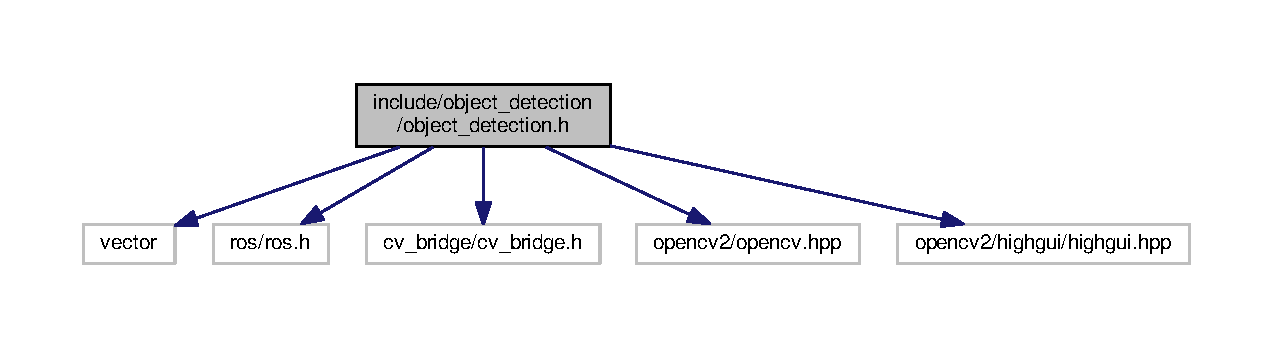
\includegraphics[width=350pt]{object__detection_8h__incl}
\end{center}
\end{figure}
This graph shows which files directly or indirectly include this file\+:
\nopagebreak
\begin{figure}[H]
\begin{center}
\leavevmode
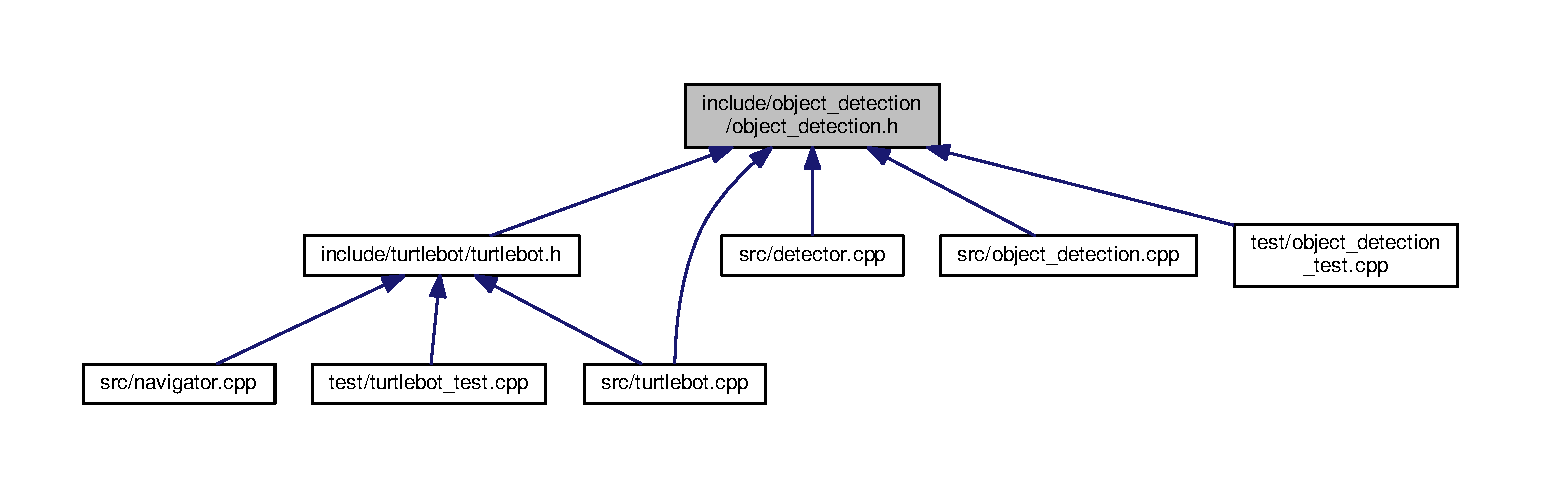
\includegraphics[width=202pt]{object__detection_8h__dep__incl}
\end{center}
\end{figure}
\subsection*{Classes}
\begin{DoxyCompactItemize}
\item 
class \hyperlink{classObjectDectection}{Object\+Dectection}
\end{DoxyCompactItemize}


\subsection{Detailed Description}
Library header file to implement object detection  Deploys template matching to detect object in the bot\textquotesingle{}s world. 

B\+SD 3-\/\+Clause License

\begin{DoxyCopyright}{Copyright}
(c) 2019, Umang Rastogi Naman Gupta All rights reserved. Redistribution and use in source and binary forms, with or without modification, are permitted provided that the following conditions are met\+:
\end{DoxyCopyright}
Redistributions of source code must retain the above copyright notice, this list of conditions and the following disclaimer. Redistributions in binary form must reproduce the above copyright notice, this list of conditions and the following disclaimer in the documentation and/or other materials provided with the distribution. Neither the name of the copyright holder nor the names of its contributors may be used to endorse or promote products derived from this software without specific prior written permission. T\+H\+IS S\+O\+F\+T\+W\+A\+RE IS P\+R\+O\+V\+I\+D\+ED BY T\+HE C\+O\+P\+Y\+R\+I\+G\+HT H\+O\+L\+D\+E\+RS A\+ND C\+O\+N\+T\+R\+I\+B\+U\+T\+O\+RS \char`\"{}\+A\+S I\+S\char`\"{} A\+ND A\+NY E\+X\+P\+R\+E\+SS OR I\+M\+P\+L\+I\+ED W\+A\+R\+R\+A\+N\+T\+I\+ES, I\+N\+C\+L\+U\+D\+I\+NG, B\+UT N\+OT L\+I\+M\+I\+T\+ED TO, T\+HE I\+M\+P\+L\+I\+ED W\+A\+R\+R\+A\+N\+T\+I\+ES OF M\+E\+R\+C\+H\+A\+N\+T\+A\+B\+I\+L\+I\+TY A\+ND F\+I\+T\+N\+E\+SS F\+OR A P\+A\+R\+T\+I\+C\+U\+L\+AR P\+U\+R\+P\+O\+SE A\+RE D\+I\+S\+C\+L\+A\+I\+M\+ED. IN NO E\+V\+E\+NT S\+H\+A\+LL T\+HE C\+O\+P\+Y\+R\+I\+G\+HT H\+O\+L\+D\+ER OR C\+O\+N\+T\+R\+I\+B\+U\+T\+O\+RS BE L\+I\+A\+B\+LE F\+OR A\+NY D\+I\+R\+E\+CT, I\+N\+D\+I\+R\+E\+CT, I\+N\+C\+I\+D\+E\+N\+T\+AL, S\+P\+E\+C\+I\+AL, E\+X\+E\+M\+P\+L\+A\+RY, OR C\+O\+N\+S\+E\+Q\+U\+E\+N\+T\+I\+AL D\+A\+M\+A\+G\+ES (I\+N\+C\+L\+U\+D\+I\+NG, B\+UT N\+OT L\+I\+M\+I\+T\+ED TO, P\+R\+O\+C\+U\+R\+E\+M\+E\+NT OF S\+U\+B\+S\+T\+I\+T\+U\+TE G\+O\+O\+DS OR S\+E\+R\+V\+I\+C\+ES; L\+O\+SS OF U\+SE, D\+A\+TA, OR P\+R\+O\+F\+I\+TS; OR B\+U\+S\+I\+N\+E\+SS I\+N\+T\+E\+R\+R\+U\+P\+T\+I\+ON) H\+O\+W\+E\+V\+ER C\+A\+U\+S\+ED A\+ND ON A\+NY T\+H\+E\+O\+RY OF L\+I\+A\+B\+I\+L\+I\+TY, W\+H\+E\+T\+H\+ER IN C\+O\+N\+T\+R\+A\+CT, S\+T\+R\+I\+CT L\+I\+A\+B\+I\+L\+I\+TY, OR T\+O\+RT (I\+N\+C\+L\+U\+D\+I\+NG N\+E\+G\+L\+I\+G\+E\+N\+CE OR O\+T\+H\+E\+R\+W\+I\+SE) A\+R\+I\+S\+I\+NG IN A\+NY W\+AY O\+UT OF T\+HE U\+SE OF T\+H\+IS S\+O\+F\+T\+W\+A\+RE, E\+V\+EN IF A\+D\+V\+I\+S\+ED OF T\+HE P\+O\+S\+S\+I\+B\+I\+L\+I\+TY OF S\+U\+CH D\+A\+M\+A\+GE.

\begin{DoxyAuthor}{Author}
Umang Rastogi -\/ Driver 

Naman Gupta -\/ Navigator 
\end{DoxyAuthor}

\hypertarget{obstacle__avoidance_8h}{}\section{include/obstacle\+\_\+avoidance/obstacle\+\_\+avoidance.h File Reference}
\label{obstacle__avoidance_8h}\index{include/obstacle\+\_\+avoidance/obstacle\+\_\+avoidance.\+h@{include/obstacle\+\_\+avoidance/obstacle\+\_\+avoidance.\+h}}


Library header file to implement obstacle avoidance.  


{\ttfamily \#include \char`\"{}ros/ros.\+h\char`\"{}}\\*
{\ttfamily \#include \char`\"{}sensor\+\_\+msgs/\+Laser\+Scan.\+h\char`\"{}}\\*
Include dependency graph for obstacle\+\_\+avoidance.\+h\+:\nopagebreak
\begin{figure}[H]
\begin{center}
\leavevmode
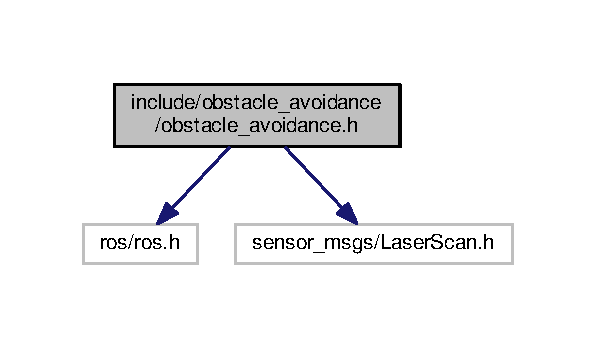
\includegraphics[width=286pt]{obstacle__avoidance_8h__incl}
\end{center}
\end{figure}
This graph shows which files directly or indirectly include this file\+:
\nopagebreak
\begin{figure}[H]
\begin{center}
\leavevmode
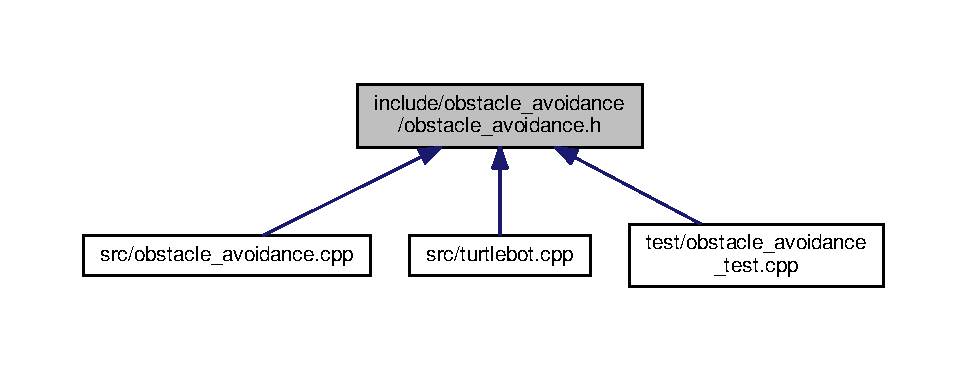
\includegraphics[width=350pt]{obstacle__avoidance_8h__dep__incl}
\end{center}
\end{figure}
\subsection*{Classes}
\begin{DoxyCompactItemize}
\item 
class \hyperlink{classObstacleAvoidance}{Obstacle\+Avoidance}
\end{DoxyCompactItemize}


\subsection{Detailed Description}
Library header file to implement obstacle avoidance. 

B\+SD 3-\/\+Clause License

\begin{DoxyCopyright}{Copyright}
(c) 2019, Umang Rastogi, Naman Gupta
\end{DoxyCopyright}
All rights reserved. Redistribution and use in source and binary forms, with or without modification, are permitted provided that the following conditions are met\+:

Redistributions of source code must retain the above copyright notice, this list of conditions and the following disclaimer. Redistributions in binary form must reproduce the above copyright notice, this list of conditions and the following disclaimer in the documentation and/or other materials provided with the distribution. Neither the name of the copyright holder nor the names of its contributors may be used to endorse or promote products derived from this software without specific prior written permission. T\+H\+IS S\+O\+F\+T\+W\+A\+RE IS P\+R\+O\+V\+I\+D\+ED BY T\+HE C\+O\+P\+Y\+R\+I\+G\+HT H\+O\+L\+D\+E\+RS A\+ND C\+O\+N\+T\+R\+I\+B\+U\+T\+O\+RS \char`\"{}\+A\+S I\+S\char`\"{} A\+ND A\+NY E\+X\+P\+R\+E\+SS OR I\+M\+P\+L\+I\+ED W\+A\+R\+R\+A\+N\+T\+I\+ES, I\+N\+C\+L\+U\+D\+I\+NG, B\+UT N\+OT L\+I\+M\+I\+T\+ED TO, T\+HE I\+M\+P\+L\+I\+ED W\+A\+R\+R\+A\+N\+T\+I\+ES OF M\+E\+R\+C\+H\+A\+N\+T\+A\+B\+I\+L\+I\+TY A\+ND F\+I\+T\+N\+E\+SS F\+OR A P\+A\+R\+T\+I\+C\+U\+L\+AR P\+U\+R\+P\+O\+SE A\+RE D\+I\+S\+C\+L\+A\+I\+M\+ED. IN NO E\+V\+E\+NT S\+H\+A\+LL T\+HE C\+O\+P\+Y\+R\+I\+G\+HT H\+O\+L\+D\+ER OR C\+O\+N\+T\+R\+I\+B\+U\+T\+O\+RS BE L\+I\+A\+B\+LE F\+OR A\+NY D\+I\+R\+E\+CT, I\+N\+D\+I\+R\+E\+CT, I\+N\+C\+I\+D\+E\+N\+T\+AL, S\+P\+E\+C\+I\+AL, E\+X\+E\+M\+P\+L\+A\+RY, OR C\+O\+N\+S\+E\+Q\+U\+E\+N\+T\+I\+AL D\+A\+M\+A\+G\+ES (I\+N\+C\+L\+U\+D\+I\+NG, B\+UT N\+OT L\+I\+M\+I\+T\+ED TO, P\+R\+O\+C\+U\+R\+E\+M\+E\+NT OF S\+U\+B\+S\+T\+I\+T\+U\+TE G\+O\+O\+DS OR S\+E\+R\+V\+I\+C\+ES; L\+O\+SS OF U\+SE, D\+A\+TA, OR P\+R\+O\+F\+I\+TS; OR B\+U\+S\+I\+N\+E\+SS I\+N\+T\+E\+R\+R\+U\+P\+T\+I\+ON) H\+O\+W\+E\+V\+ER C\+A\+U\+S\+ED A\+ND ON A\+NY T\+H\+E\+O\+RY OF L\+I\+A\+B\+I\+L\+I\+TY, W\+H\+E\+T\+H\+ER IN C\+O\+N\+T\+R\+A\+CT, S\+T\+R\+I\+CT L\+I\+A\+B\+I\+L\+I\+TY, OR T\+O\+RT (I\+N\+C\+L\+U\+D\+I\+NG N\+E\+G\+L\+I\+G\+E\+N\+CE OR O\+T\+H\+E\+R\+W\+I\+SE) A\+R\+I\+S\+I\+NG IN A\+NY W\+AY O\+UT OF T\+HE U\+SE OF T\+H\+IS S\+O\+F\+T\+W\+A\+RE, E\+V\+EN IF A\+D\+V\+I\+S\+ED OF T\+HE P\+O\+S\+S\+I\+B\+I\+L\+I\+TY OF S\+U\+CH D\+A\+M\+A\+GE.

\begin{DoxyAuthor}{Author}
Umang Rastogi -\/ Driver 

Naman Gupta -\/ Navigator 
\end{DoxyAuthor}

\hypertarget{turtlebot_8h}{}\section{include/turtlebot/turtlebot.h File Reference}
\label{turtlebot_8h}\index{include/turtlebot/turtlebot.\+h@{include/turtlebot/turtlebot.\+h}}


Library header file to control motion of the bot  Takes input from both, obstacle avoidance and object detection.  


{\ttfamily \#include \char`\"{}ros/ros.\+h\char`\"{}}\\*
{\ttfamily \#include \char`\"{}geometry\+\_\+msgs/\+Twist.\+h\char`\"{}}\\*
Include dependency graph for turtlebot.\+h\+:
\nopagebreak
\begin{figure}[H]
\begin{center}
\leavevmode
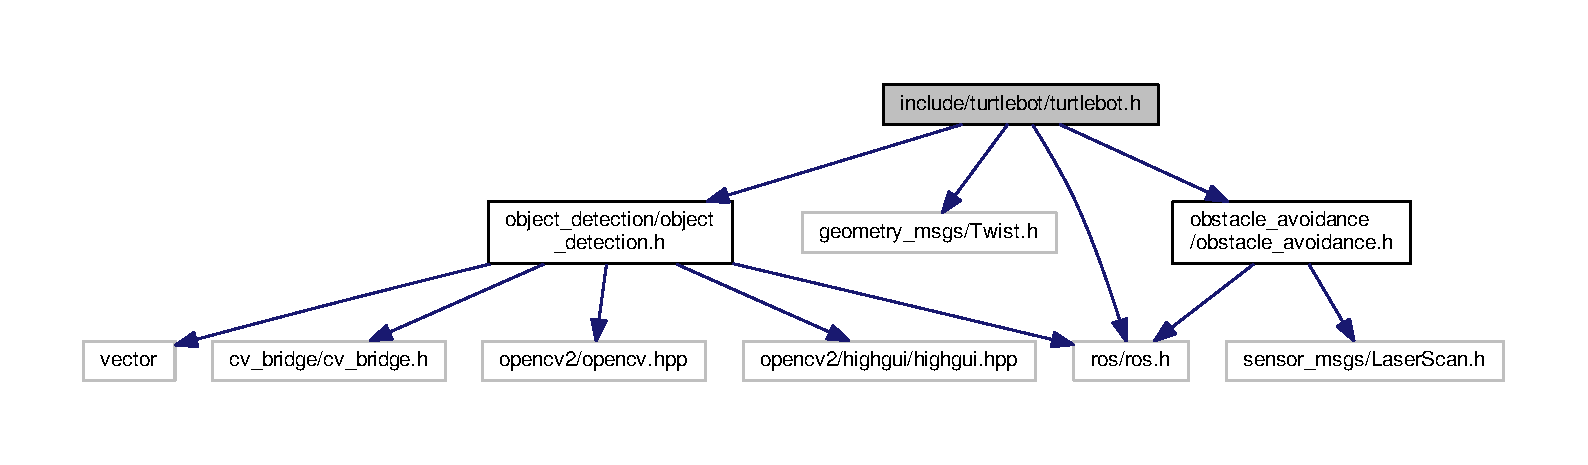
\includegraphics[width=276pt]{turtlebot_8h__incl}
\end{center}
\end{figure}
This graph shows which files directly or indirectly include this file\+:
\nopagebreak
\begin{figure}[H]
\begin{center}
\leavevmode
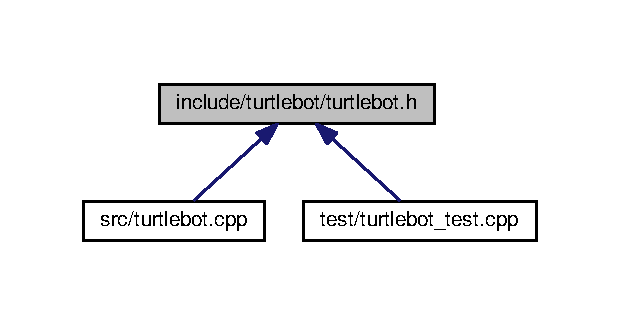
\includegraphics[width=298pt]{turtlebot_8h__dep__incl}
\end{center}
\end{figure}
\subsection*{Classes}
\begin{DoxyCompactItemize}
\item 
class \hyperlink{classTurtlebot}{Turtlebot}
\begin{DoxyCompactList}\small\item\em Add R\+OS headers. \end{DoxyCompactList}\end{DoxyCompactItemize}


\subsection{Detailed Description}
Library header file to control motion of the bot  Takes input from both, obstacle avoidance and object detection. 

B\+SD 3-\/\+Clause License

\begin{DoxyCopyright}{Copyright}
(c) 2019, Umang Rastogi Naman Gupta All rights reserved. Redistribution and use in source and binary forms, with or without modification, are permitted provided that the following conditions are met\+:
\end{DoxyCopyright}
Redistributions of source code must retain the above copyright notice, this list of conditions and the following disclaimer. Redistributions in binary form must reproduce the above copyright notice, this list of conditions and the following disclaimer in the documentation and/or other materials provided with the distribution. Neither the name of the copyright holder nor the names of its contributors may be used to endorse or promote products derived from this software without specific prior written permission. T\+H\+IS S\+O\+F\+T\+W\+A\+RE IS P\+R\+O\+V\+I\+D\+ED BY T\+HE C\+O\+P\+Y\+R\+I\+G\+HT H\+O\+L\+D\+E\+RS A\+ND C\+O\+N\+T\+R\+I\+B\+U\+T\+O\+RS \char`\"{}\+A\+S I\+S\char`\"{} A\+ND A\+NY E\+X\+P\+R\+E\+SS OR I\+M\+P\+L\+I\+ED W\+A\+R\+R\+A\+N\+T\+I\+ES, I\+N\+C\+L\+U\+D\+I\+NG, B\+UT N\+OT L\+I\+M\+I\+T\+ED TO, T\+HE I\+M\+P\+L\+I\+ED W\+A\+R\+R\+A\+N\+T\+I\+ES OF M\+E\+R\+C\+H\+A\+N\+T\+A\+B\+I\+L\+I\+TY A\+ND F\+I\+T\+N\+E\+SS F\+OR A P\+A\+R\+T\+I\+C\+U\+L\+AR P\+U\+R\+P\+O\+SE A\+RE D\+I\+S\+C\+L\+A\+I\+M\+ED. IN NO E\+V\+E\+NT S\+H\+A\+LL T\+HE C\+O\+P\+Y\+R\+I\+G\+HT H\+O\+L\+D\+ER OR C\+O\+N\+T\+R\+I\+B\+U\+T\+O\+RS BE L\+I\+A\+B\+LE F\+OR A\+NY D\+I\+R\+E\+CT, I\+N\+D\+I\+R\+E\+CT, I\+N\+C\+I\+D\+E\+N\+T\+AL, S\+P\+E\+C\+I\+AL, E\+X\+E\+M\+P\+L\+A\+RY, OR C\+O\+N\+S\+E\+Q\+U\+E\+N\+T\+I\+AL D\+A\+M\+A\+G\+ES (I\+N\+C\+L\+U\+D\+I\+NG, B\+UT N\+OT L\+I\+M\+I\+T\+ED TO, P\+R\+O\+C\+U\+R\+E\+M\+E\+NT OF S\+U\+B\+S\+T\+I\+T\+U\+TE G\+O\+O\+DS OR S\+E\+R\+V\+I\+C\+ES; L\+O\+SS OF U\+SE, D\+A\+TA, OR P\+R\+O\+F\+I\+TS; OR B\+U\+S\+I\+N\+E\+SS I\+N\+T\+E\+R\+R\+U\+P\+T\+I\+ON) H\+O\+W\+E\+V\+ER C\+A\+U\+S\+ED A\+ND ON A\+NY T\+H\+E\+O\+RY OF L\+I\+A\+B\+I\+L\+I\+TY, W\+H\+E\+T\+H\+ER IN C\+O\+N\+T\+R\+A\+CT, S\+T\+R\+I\+CT L\+I\+A\+B\+I\+L\+I\+TY, OR T\+O\+RT (I\+N\+C\+L\+U\+D\+I\+NG N\+E\+G\+L\+I\+G\+E\+N\+CE OR O\+T\+H\+E\+R\+W\+I\+SE) A\+R\+I\+S\+I\+NG IN A\+NY W\+AY O\+UT OF T\+HE U\+SE OF T\+H\+IS S\+O\+F\+T\+W\+A\+RE, E\+V\+EN IF A\+D\+V\+I\+S\+ED OF T\+HE P\+O\+S\+S\+I\+B\+I\+L\+I\+TY OF S\+U\+CH D\+A\+M\+A\+GE.

\begin{DoxyAuthor}{Author}
Umang Rastogi -\/ Driver 

Naman Gupta -\/ Navigator 
\end{DoxyAuthor}

\hypertarget{README_8md}{}\section{R\+E\+A\+D\+M\+E.\+md File Reference}
\label{README_8md}\index{R\+E\+A\+D\+M\+E.\+md@{R\+E\+A\+D\+M\+E.\+md}}

\hypertarget{detector_8cpp}{}\section{src/detector.cpp File Reference}
\label{detector_8cpp}\index{src/detector.\+cpp@{src/detector.\+cpp}}


Detector node file to implement object detection algorithm  Implements object detection algorithm using H\+SV color detection.  


{\ttfamily \#include $<$ros/ros.\+h$>$}\\*
{\ttfamily \#include \char`\"{}object\+\_\+detection/object\+\_\+detection.\+h\char`\"{}}\\*
Include dependency graph for detector.\+cpp\+:
\nopagebreak
\begin{figure}[H]
\begin{center}
\leavevmode
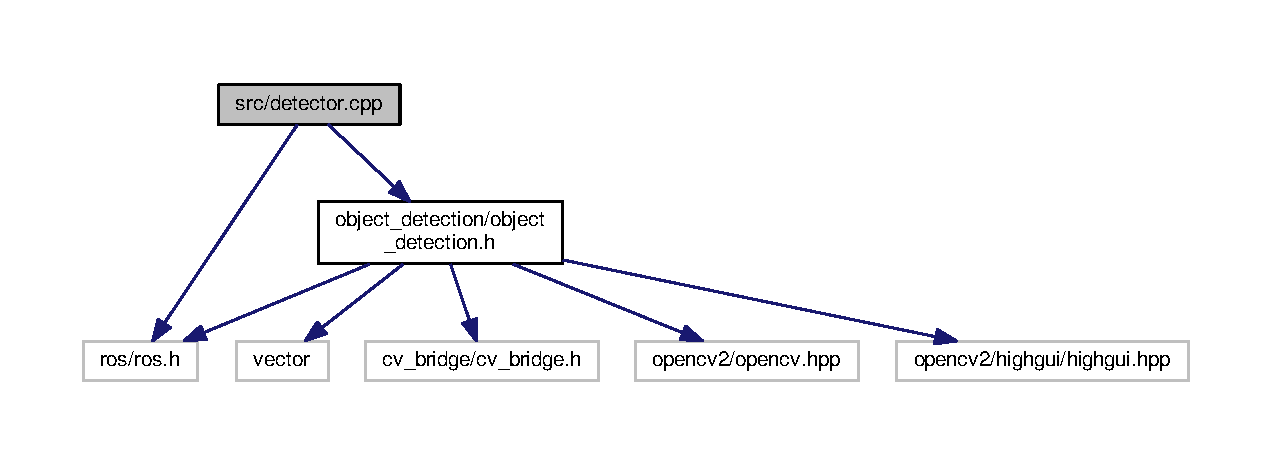
\includegraphics[width=350pt]{detector_8cpp__incl}
\end{center}
\end{figure}
\subsection*{Functions}
\begin{DoxyCompactItemize}
\item 
int \hyperlink{detector_8cpp_a3c04138a5bfe5d72780bb7e82a18e627}{main} (int argc, char $\ast$$\ast$argv)
\begin{DoxyCompactList}\small\item\em main function \end{DoxyCompactList}\end{DoxyCompactItemize}


\subsection{Detailed Description}
Detector node file to implement object detection algorithm  Implements object detection algorithm using H\+SV color detection. 

B\+SD 3-\/\+Clause License

\begin{DoxyCopyright}{Copyright}
(c) 2019, Umang Rastogi, Naman Gupta
\end{DoxyCopyright}
All rights reserved. Redistribution and use in source and binary forms, with or without modification, are permitted provided that the following conditions are met\+:

Redistributions of source code must retain the above copyright notice, this list of conditions and the following disclaimer. Redistributions in binary form must reproduce the above copyright notice, this list of conditions and the following disclaimer in the documentation and/or other materials provided with the distribution. Neither the name of the copyright holder nor the names of its contributors may be used to endorse or promote products derived from this software without specific prior written permission. T\+H\+IS S\+O\+F\+T\+W\+A\+RE IS P\+R\+O\+V\+I\+D\+ED BY T\+HE C\+O\+P\+Y\+R\+I\+G\+HT H\+O\+L\+D\+E\+RS A\+ND C\+O\+N\+T\+R\+I\+B\+U\+T\+O\+RS \char`\"{}\+A\+S I\+S\char`\"{} A\+ND A\+NY E\+X\+P\+R\+E\+SS OR I\+M\+P\+L\+I\+ED W\+A\+R\+R\+A\+N\+T\+I\+ES, I\+N\+C\+L\+U\+D\+I\+NG, B\+UT N\+OT L\+I\+M\+I\+T\+ED TO, T\+HE I\+M\+P\+L\+I\+ED W\+A\+R\+R\+A\+N\+T\+I\+ES OF M\+E\+R\+C\+H\+A\+N\+T\+A\+B\+I\+L\+I\+TY A\+ND F\+I\+T\+N\+E\+SS F\+OR A P\+A\+R\+T\+I\+C\+U\+L\+AR P\+U\+R\+P\+O\+SE A\+RE D\+I\+S\+C\+L\+A\+I\+M\+ED. IN NO E\+V\+E\+NT S\+H\+A\+LL T\+HE C\+O\+P\+Y\+R\+I\+G\+HT H\+O\+L\+D\+ER OR C\+O\+N\+T\+R\+I\+B\+U\+T\+O\+RS BE L\+I\+A\+B\+LE F\+OR A\+NY D\+I\+R\+E\+CT, I\+N\+D\+I\+R\+E\+CT, I\+N\+C\+I\+D\+E\+N\+T\+AL, S\+P\+E\+C\+I\+AL, E\+X\+E\+M\+P\+L\+A\+RY, OR C\+O\+N\+S\+E\+Q\+U\+E\+N\+T\+I\+AL D\+A\+M\+A\+G\+ES (I\+N\+C\+L\+U\+D\+I\+NG, B\+UT N\+OT L\+I\+M\+I\+T\+ED TO, P\+R\+O\+C\+U\+R\+E\+M\+E\+NT OF S\+U\+B\+S\+T\+I\+T\+U\+TE G\+O\+O\+DS OR S\+E\+R\+V\+I\+C\+ES; L\+O\+SS OF U\+SE, D\+A\+TA, OR P\+R\+O\+F\+I\+TS; OR B\+U\+S\+I\+N\+E\+SS I\+N\+T\+E\+R\+R\+U\+P\+T\+I\+ON) H\+O\+W\+E\+V\+ER C\+A\+U\+S\+ED A\+ND ON A\+NY T\+H\+E\+O\+RY OF L\+I\+A\+B\+I\+L\+I\+TY, W\+H\+E\+T\+H\+ER IN C\+O\+N\+T\+R\+A\+CT, S\+T\+R\+I\+CT L\+I\+A\+B\+I\+L\+I\+TY, OR T\+O\+RT (I\+N\+C\+L\+U\+D\+I\+NG N\+E\+G\+L\+I\+G\+E\+N\+CE OR O\+T\+H\+E\+R\+W\+I\+SE) A\+R\+I\+S\+I\+NG IN A\+NY W\+AY O\+UT OF T\+HE U\+SE OF T\+H\+IS S\+O\+F\+T\+W\+A\+RE, E\+V\+EN IF A\+D\+V\+I\+S\+ED OF T\+HE P\+O\+S\+S\+I\+B\+I\+L\+I\+TY OF S\+U\+CH D\+A\+M\+A\+GE.

\begin{DoxyAuthor}{Author}
Umang Rastogi -\/ Navigator 

Naman Gupta -\/ Driver 
\end{DoxyAuthor}


\subsection{Function Documentation}
\index{detector.\+cpp@{detector.\+cpp}!main@{main}}
\index{main@{main}!detector.\+cpp@{detector.\+cpp}}
\subsubsection[{\texorpdfstring{main(int argc, char $\ast$$\ast$argv)}{main(int argc, char **argv)}}]{\setlength{\rightskip}{0pt plus 5cm}int main (
\begin{DoxyParamCaption}
\item[{int}]{argc, }
\item[{char $\ast$$\ast$}]{argv}
\end{DoxyParamCaption}
)}\hypertarget{detector_8cpp_a3c04138a5bfe5d72780bb7e82a18e627}{}\label{detector_8cpp_a3c04138a5bfe5d72780bb7e82a18e627}


main function 


\begin{DoxyParams}{Parameters}
{\em argc} & \\
\hline
{\em argv} & \\
\hline
\end{DoxyParams}
\begin{DoxyReturn}{Returns}
int 
\end{DoxyReturn}
Initialized object detection node

Declaring object of class \hyperlink{classObjectDetection}{Object\+Detection}

Checks empty image

Apply detect\+Object method to detect cans in the world

Close both the windows of H\+S\+V\+Image and \hyperlink{classTurtlebot}{Turtlebot} View 
\hypertarget{navigator_8cpp}{}\section{src/navigator.cpp File Reference}
\label{navigator_8cpp}\index{src/navigator.\+cpp@{src/navigator.\+cpp}}
{\ttfamily \#include \char`\"{}ros/ros.\+h\char`\"{}}\\*
{\ttfamily \#include \char`\"{}turtlebot/turtlebot.\+h\char`\"{}}\\*
{\ttfamily \#include \char`\"{}obstacle\+\_\+avoidance/obstacle\+\_\+avoidance.\+h\char`\"{}}\\*
Include dependency graph for navigator.\+cpp\+:
\nopagebreak
\begin{figure}[H]
\begin{center}
\leavevmode
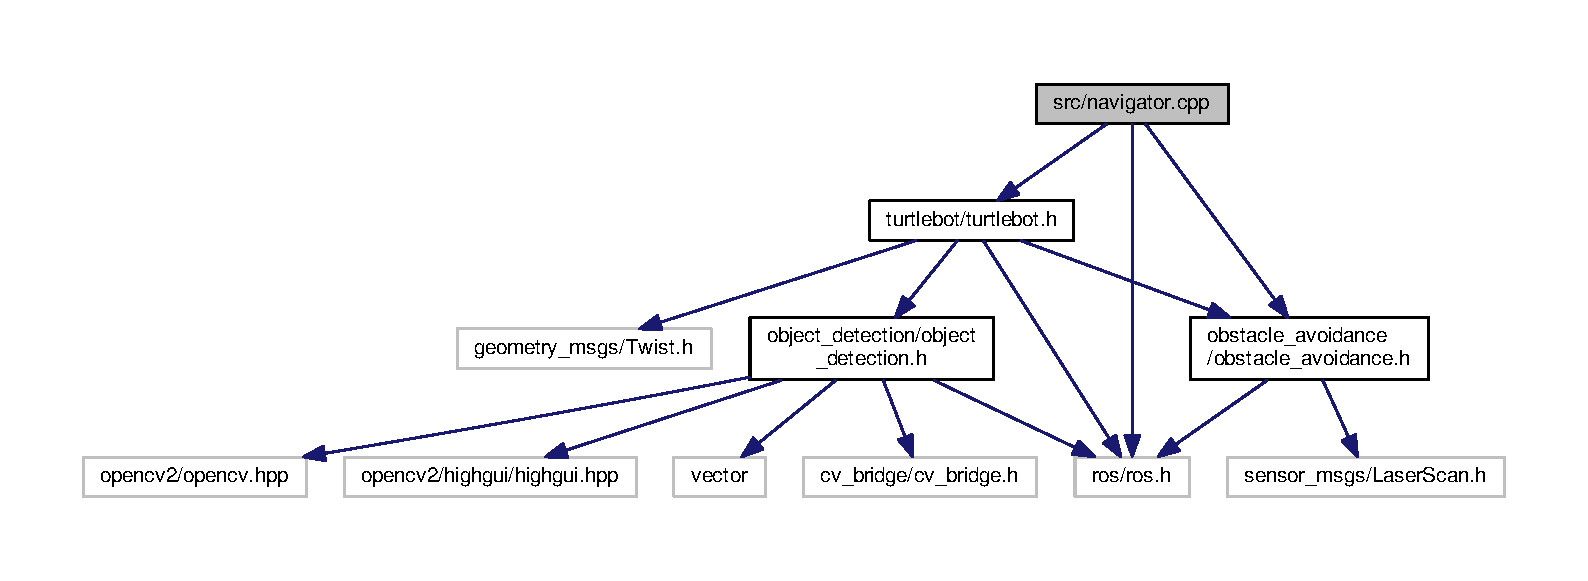
\includegraphics[width=350pt]{navigator_8cpp__incl}
\end{center}
\end{figure}
\subsection*{Functions}
\begin{DoxyCompactItemize}
\item 
int \hyperlink{navigator_8cpp_a0ddf1224851353fc92bfbff6f499fa97}{main} (int argc, char $\ast$argv\mbox{[}$\,$\mbox{]})
\begin{DoxyCompactList}\small\item\em main function \end{DoxyCompactList}\end{DoxyCompactItemize}


\subsection{Function Documentation}
\index{navigator.\+cpp@{navigator.\+cpp}!main@{main}}
\index{main@{main}!navigator.\+cpp@{navigator.\+cpp}}
\subsubsection[{\texorpdfstring{main(int argc, char $\ast$argv[])}{main(int argc, char *argv[])}}]{\setlength{\rightskip}{0pt plus 5cm}int main (
\begin{DoxyParamCaption}
\item[{int}]{argc, }
\item[{char $\ast$}]{argv\mbox{[}$\,$\mbox{]}}
\end{DoxyParamCaption}
)}\hypertarget{navigator_8cpp_a0ddf1224851353fc92bfbff6f499fa97}{}\label{navigator_8cpp_a0ddf1224851353fc92bfbff6f499fa97}


main function 


\begin{DoxyParams}{Parameters}
{\em argc} & \\
\hline
{\em argv} & \\
\hline
\end{DoxyParams}
\begin{DoxyReturn}{Returns}
int 
\end{DoxyReturn}
Initialized object collection node

Declaring object of class \hyperlink{classObstacleAvoidance}{Obstacle\+Avoidance}

Declaring object of class \hyperlink{classTurtlebot}{Turtlebot}

Starts moving the bot 
\hypertarget{object__detection_8cpp}{}\section{src/object\+\_\+detection.cpp File Reference}
\label{object__detection_8cpp}\index{src/object\+\_\+detection.\+cpp@{src/object\+\_\+detection.\+cpp}}


File to implement \hyperlink{classObjectDetection}{Object\+Detection} class  Implements object detection using H\+SV method which detects color of the can in a certain range and creates a bounding box over it.  


{\ttfamily \#include \char`\"{}ros/ros.\+h\char`\"{}}\\*
{\ttfamily \#include \char`\"{}sensor\+\_\+msgs/\+Image.\+h\char`\"{}}\\*
{\ttfamily \#include \char`\"{}cv\+\_\+bridge/cv\+\_\+bridge.\+h\char`\"{}}\\*
{\ttfamily \#include \char`\"{}object\+\_\+detection/object\+\_\+detection.\+h\char`\"{}}\\*
{\ttfamily \#include \char`\"{}opencv2/highgui/highgui.\+hpp\char`\"{}}\\*
{\ttfamily \#include \char`\"{}opencv2/imgproc/imgproc.\+hpp\char`\"{}}\\*
Include dependency graph for object\+\_\+detection.\+cpp\+:
\nopagebreak
\begin{figure}[H]
\begin{center}
\leavevmode
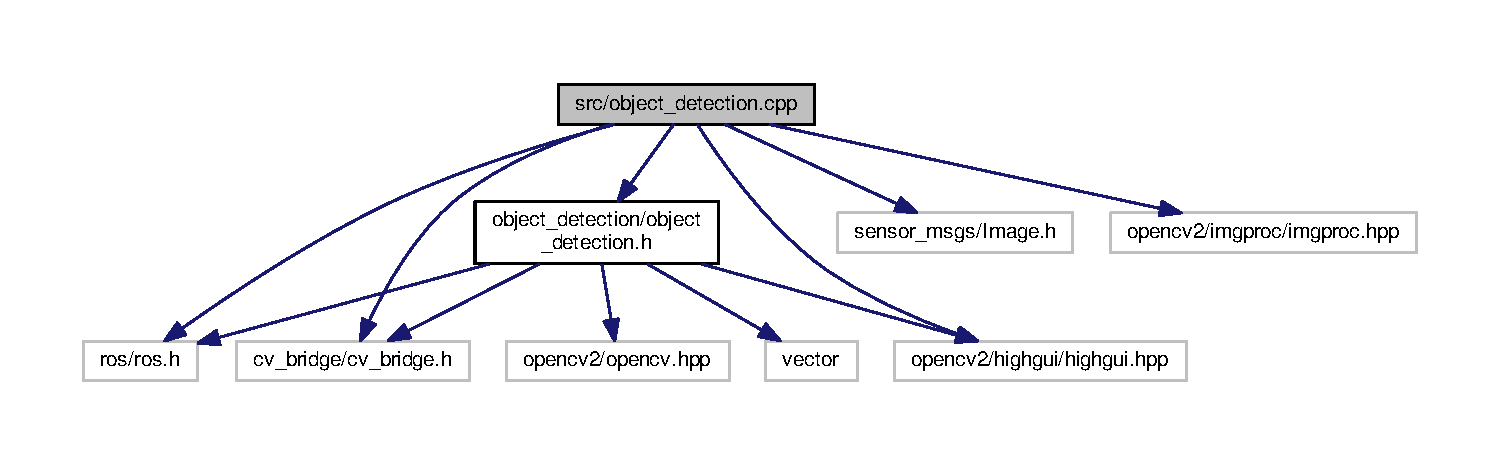
\includegraphics[width=350pt]{object__detection_8cpp__incl}
\end{center}
\end{figure}


\subsection{Detailed Description}
File to implement \hyperlink{classObjectDetection}{Object\+Detection} class  Implements object detection using H\+SV method which detects color of the can in a certain range and creates a bounding box over it. 

B\+SD 3-\/\+Clause License

\begin{DoxyCopyright}{Copyright}
(c) 2019, Umang Rastogi Naman Gupta All rights reserved. Redistribution and use in source and binary forms, with or without modification, are permitted provided that the following conditions are met\+:
\end{DoxyCopyright}
Redistributions of source code must retain the above copyright notice, this list of conditions and the following disclaimer. Redistributions in binary form must reproduce the above copyright notice, this list of conditions and the following disclaimer in the documentation and/or other materials provided with the distribution. Neither the name of the copyright holder nor the names of its contributors may be used to endorse or promote products derived from this software without specific prior written permission. T\+H\+IS S\+O\+F\+T\+W\+A\+RE IS P\+R\+O\+V\+I\+D\+ED BY T\+HE C\+O\+P\+Y\+R\+I\+G\+HT H\+O\+L\+D\+E\+RS A\+ND C\+O\+N\+T\+R\+I\+B\+U\+T\+O\+RS \char`\"{}\+A\+S I\+S\char`\"{} A\+ND A\+NY E\+X\+P\+R\+E\+SS OR I\+M\+P\+L\+I\+ED W\+A\+R\+R\+A\+N\+T\+I\+ES, I\+N\+C\+L\+U\+D\+I\+NG, B\+UT N\+OT L\+I\+M\+I\+T\+ED TO, T\+HE I\+M\+P\+L\+I\+ED W\+A\+R\+R\+A\+N\+T\+I\+ES OF M\+E\+R\+C\+H\+A\+N\+T\+A\+B\+I\+L\+I\+TY A\+ND F\+I\+T\+N\+E\+SS F\+OR A P\+A\+R\+T\+I\+C\+U\+L\+AR P\+U\+R\+P\+O\+SE A\+RE D\+I\+S\+C\+L\+A\+I\+M\+ED. IN NO E\+V\+E\+NT S\+H\+A\+LL T\+HE C\+O\+P\+Y\+R\+I\+G\+HT H\+O\+L\+D\+ER OR C\+O\+N\+T\+R\+I\+B\+U\+T\+O\+RS BE L\+I\+A\+B\+LE F\+OR A\+NY D\+I\+R\+E\+CT, I\+N\+D\+I\+R\+E\+CT, I\+N\+C\+I\+D\+E\+N\+T\+AL, S\+P\+E\+C\+I\+AL, E\+X\+E\+M\+P\+L\+A\+RY, OR C\+O\+N\+S\+E\+Q\+U\+E\+N\+T\+I\+AL D\+A\+M\+A\+G\+ES (I\+N\+C\+L\+U\+D\+I\+NG, B\+UT N\+OT L\+I\+M\+I\+T\+ED TO, P\+R\+O\+C\+U\+R\+E\+M\+E\+NT OF S\+U\+B\+S\+T\+I\+T\+U\+TE G\+O\+O\+DS OR S\+E\+R\+V\+I\+C\+ES; L\+O\+SS OF U\+SE, D\+A\+TA, OR P\+R\+O\+F\+I\+TS; OR B\+U\+S\+I\+N\+E\+SS I\+N\+T\+E\+R\+R\+U\+P\+T\+I\+ON) H\+O\+W\+E\+V\+ER C\+A\+U\+S\+ED A\+ND ON A\+NY T\+H\+E\+O\+RY OF L\+I\+A\+B\+I\+L\+I\+TY, W\+H\+E\+T\+H\+ER IN C\+O\+N\+T\+R\+A\+CT, S\+T\+R\+I\+CT L\+I\+A\+B\+I\+L\+I\+TY, OR T\+O\+RT (I\+N\+C\+L\+U\+D\+I\+NG N\+E\+G\+L\+I\+G\+E\+N\+CE OR O\+T\+H\+E\+R\+W\+I\+SE) A\+R\+I\+S\+I\+NG IN A\+NY W\+AY O\+UT OF T\+HE U\+SE OF T\+H\+IS S\+O\+F\+T\+W\+A\+RE, E\+V\+EN IF A\+D\+V\+I\+S\+ED OF T\+HE P\+O\+S\+S\+I\+B\+I\+L\+I\+TY OF S\+U\+CH D\+A\+M\+A\+GE.

\begin{DoxyAuthor}{Author}
Umang Rastogi -\/ Driver 

Naman Gupta -\/ Navigator 
\end{DoxyAuthor}

\hypertarget{obstacle__avoidance_8cpp}{}\section{src/obstacle\+\_\+avoidance.cpp File Reference}
\label{obstacle__avoidance_8cpp}\index{src/obstacle\+\_\+avoidance.\+cpp@{src/obstacle\+\_\+avoidance.\+cpp}}
{\ttfamily \#include \char`\"{}ros/ros.\+h\char`\"{}}\\*
{\ttfamily \#include \char`\"{}geometry\+\_\+msgs/\+Twist.\+h\char`\"{}}\\*
{\ttfamily \#include \char`\"{}sensor\+\_\+msgs/\+Laser\+Scan.\+h\char`\"{}}\\*
{\ttfamily \#include \char`\"{}obstacle\+\_\+avoidance/obstacle\+\_\+avoidance.\+h\char`\"{}}\\*
Include dependency graph for obstacle\+\_\+avoidance.\+cpp\+:
\nopagebreak
\begin{figure}[H]
\begin{center}
\leavevmode
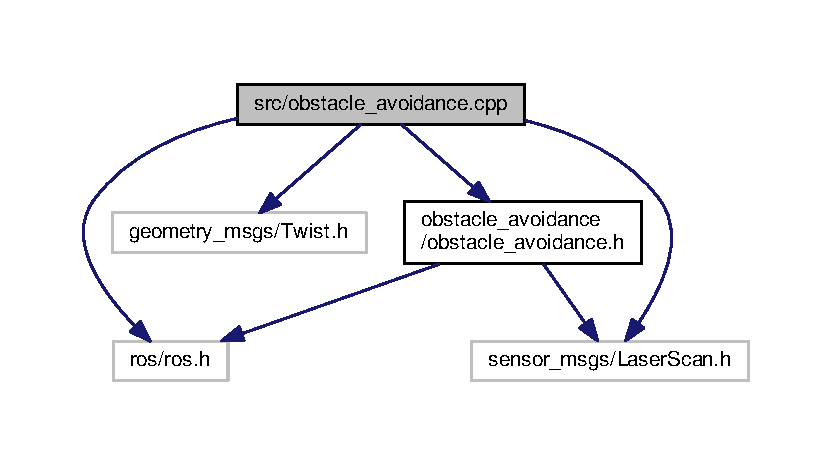
\includegraphics[width=350pt]{obstacle__avoidance_8cpp__incl}
\end{center}
\end{figure}

\hypertarget{turtlebot_8cpp}{}\section{src/turtlebot.cpp File Reference}
\label{turtlebot_8cpp}\index{src/turtlebot.\+cpp@{src/turtlebot.\+cpp}}


Navigator node to implement obstacle avoidance and move bot algorithm.  


{\ttfamily \#include \char`\"{}ros/ros.\+h\char`\"{}}\\*
{\ttfamily \#include \char`\"{}geometry\+\_\+msgs/\+Twist.\+h\char`\"{}}\\*
{\ttfamily \#include \char`\"{}turtlebot/turtlebot.\+h\char`\"{}}\\*
{\ttfamily \#include \char`\"{}object\+\_\+detection/object\+\_\+detection.\+h\char`\"{}}\\*
{\ttfamily \#include \char`\"{}obstacle\+\_\+avoidance/obstacle\+\_\+avoidance.\+h\char`\"{}}\\*
Include dependency graph for turtlebot.\+cpp\+:
\nopagebreak
\begin{figure}[H]
\begin{center}
\leavevmode
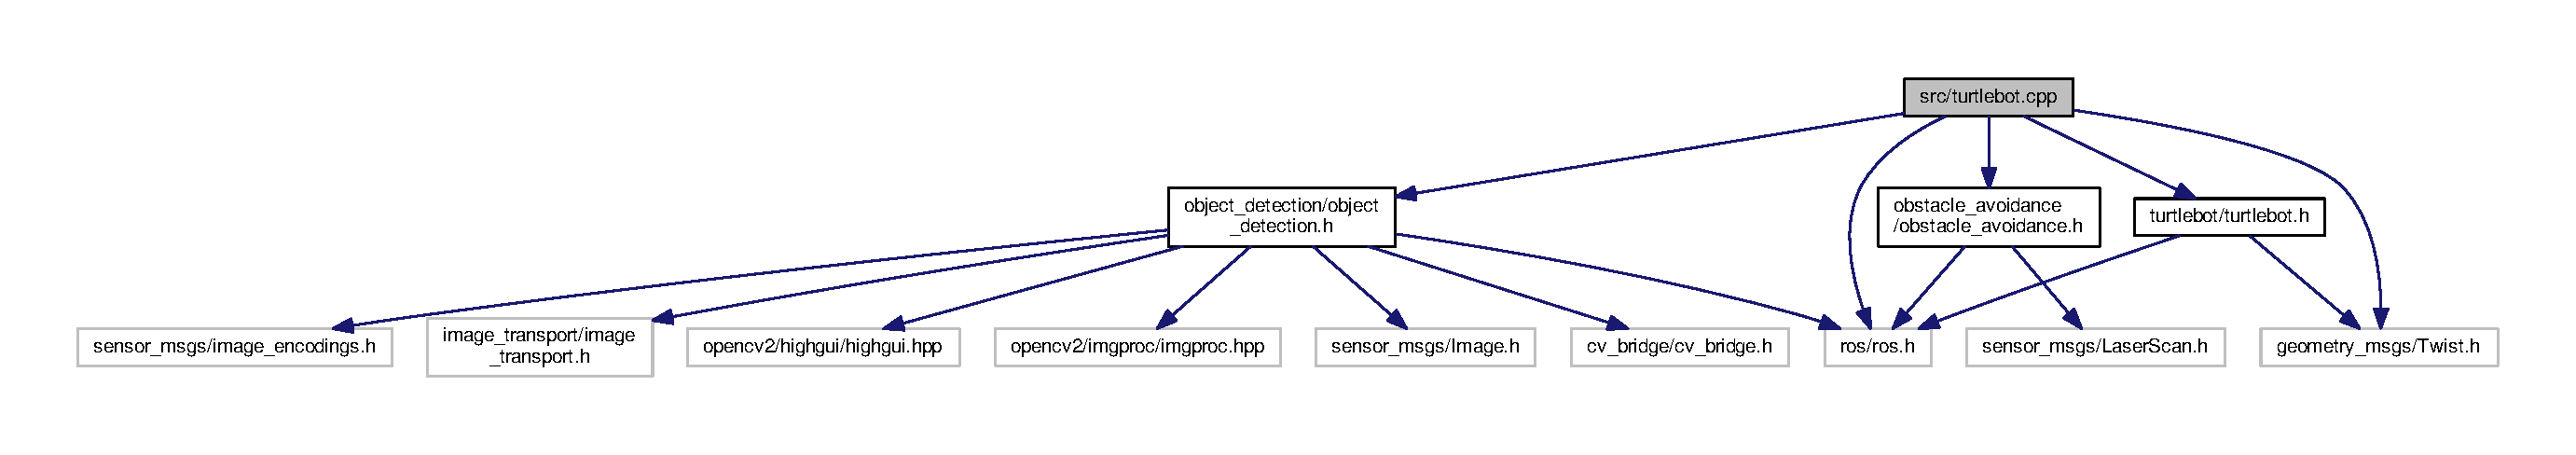
\includegraphics[width=350pt]{turtlebot_8cpp__incl}
\end{center}
\end{figure}


\subsection{Detailed Description}
Navigator node to implement obstacle avoidance and move bot algorithm. 

Source file to implement turtlebot class  Controls the motion of the bot using obstacle avoidance and go-\/to-\/goal strategies.

B\+SD 3-\/\+Clause License

\begin{DoxyCopyright}{Copyright}
(c) 2019, Naman Gupta, Umang Rastogi All rights reserved. Redistribution and use in source and binary forms, with or without modification, are permitted provided that the following conditions are met\+:
\end{DoxyCopyright}
Redistributions of source code must retain the above copyright notice, this list of conditions and the following disclaimer. Redistributions in binary form must reproduce the above copyright notice, this list of conditions and the following disclaimer in the documentation and/or other materials provided with the distribution. Neither the name of the copyright holder nor the names of its contributors may be used to endorse or promote products derived from this software without specific prior written permission. T\+H\+IS S\+O\+F\+T\+W\+A\+RE IS P\+R\+O\+V\+I\+D\+ED BY T\+HE C\+O\+P\+Y\+R\+I\+G\+HT H\+O\+L\+D\+E\+RS A\+ND C\+O\+N\+T\+R\+I\+B\+U\+T\+O\+RS \char`\"{}\+A\+S I\+S\char`\"{} A\+ND A\+NY E\+X\+P\+R\+E\+SS OR I\+M\+P\+L\+I\+ED W\+A\+R\+R\+A\+N\+T\+I\+ES, I\+N\+C\+L\+U\+D\+I\+NG, B\+UT N\+OT L\+I\+M\+I\+T\+ED TO, T\+HE I\+M\+P\+L\+I\+ED W\+A\+R\+R\+A\+N\+T\+I\+ES OF M\+E\+R\+C\+H\+A\+N\+T\+A\+B\+I\+L\+I\+TY A\+ND F\+I\+T\+N\+E\+SS F\+OR A P\+A\+R\+T\+I\+C\+U\+L\+AR P\+U\+R\+P\+O\+SE A\+RE D\+I\+S\+C\+L\+A\+I\+M\+ED. IN NO E\+V\+E\+NT S\+H\+A\+LL T\+HE C\+O\+P\+Y\+R\+I\+G\+HT H\+O\+L\+D\+ER OR C\+O\+N\+T\+R\+I\+B\+U\+T\+O\+RS BE L\+I\+A\+B\+LE F\+OR A\+NY D\+I\+R\+E\+CT, I\+N\+D\+I\+R\+E\+CT, I\+N\+C\+I\+D\+E\+N\+T\+AL, S\+P\+E\+C\+I\+AL, E\+X\+E\+M\+P\+L\+A\+RY, OR C\+O\+N\+S\+E\+Q\+U\+E\+N\+T\+I\+AL D\+A\+M\+A\+G\+ES (I\+N\+C\+L\+U\+D\+I\+NG, B\+UT N\+OT L\+I\+M\+I\+T\+ED TO, P\+R\+O\+C\+U\+R\+E\+M\+E\+NT OF S\+U\+B\+S\+T\+I\+T\+U\+TE G\+O\+O\+DS OR S\+E\+R\+V\+I\+C\+ES; L\+O\+SS OF U\+SE, D\+A\+TA, OR P\+R\+O\+F\+I\+TS; OR B\+U\+S\+I\+N\+E\+SS I\+N\+T\+E\+R\+R\+U\+P\+T\+I\+ON) H\+O\+W\+E\+V\+ER C\+A\+U\+S\+ED A\+ND ON A\+NY T\+H\+E\+O\+RY OF L\+I\+A\+B\+I\+L\+I\+TY, W\+H\+E\+T\+H\+ER IN C\+O\+N\+T\+R\+A\+CT, S\+T\+R\+I\+CT L\+I\+A\+B\+I\+L\+I\+TY, OR T\+O\+RT (I\+N\+C\+L\+U\+D\+I\+NG N\+E\+G\+L\+I\+G\+E\+N\+CE OR O\+T\+H\+E\+R\+W\+I\+SE) A\+R\+I\+S\+I\+NG IN A\+NY W\+AY O\+UT OF T\+HE U\+SE OF T\+H\+IS S\+O\+F\+T\+W\+A\+RE, E\+V\+EN IF A\+D\+V\+I\+S\+ED OF T\+HE P\+O\+S\+S\+I\+B\+I\+L\+I\+TY OF S\+U\+CH D\+A\+M\+A\+GE.

\begin{DoxyAuthor}{Author}
Umang Rastogi -\/ Driver 

Naman Gupta -\/ Navigator
\end{DoxyAuthor}
B\+SD 3-\/\+Clause License

\begin{DoxyCopyright}{Copyright}
(c) 2019, Umang Rastogi, Naman Gupta All rights reserved. Redistribution and use in source and binary forms, with or without modification, are permitted provided that the following conditions are met\+:
\end{DoxyCopyright}
Redistributions of source code must retain the above copyright notice, this list of conditions and the following disclaimer. Redistributions in binary form must reproduce the above copyright notice, this list of conditions and the following disclaimer in the documentation and/or other materials provided with the distribution. Neither the name of the copyright holder nor the names of its contributors may be used to endorse or promote products derived from this software without specific prior written permission. T\+H\+IS S\+O\+F\+T\+W\+A\+RE IS P\+R\+O\+V\+I\+D\+ED BY T\+HE C\+O\+P\+Y\+R\+I\+G\+HT H\+O\+L\+D\+E\+RS A\+ND C\+O\+N\+T\+R\+I\+B\+U\+T\+O\+RS \char`\"{}\+A\+S I\+S\char`\"{} A\+ND A\+NY E\+X\+P\+R\+E\+SS OR I\+M\+P\+L\+I\+ED W\+A\+R\+R\+A\+N\+T\+I\+ES, I\+N\+C\+L\+U\+D\+I\+NG, B\+UT N\+OT L\+I\+M\+I\+T\+ED TO, T\+HE I\+M\+P\+L\+I\+ED W\+A\+R\+R\+A\+N\+T\+I\+ES OF M\+E\+R\+C\+H\+A\+N\+T\+A\+B\+I\+L\+I\+TY A\+ND F\+I\+T\+N\+E\+SS F\+OR A P\+A\+R\+T\+I\+C\+U\+L\+AR P\+U\+R\+P\+O\+SE A\+RE D\+I\+S\+C\+L\+A\+I\+M\+ED. IN NO E\+V\+E\+NT S\+H\+A\+LL T\+HE C\+O\+P\+Y\+R\+I\+G\+HT H\+O\+L\+D\+ER OR C\+O\+N\+T\+R\+I\+B\+U\+T\+O\+RS BE L\+I\+A\+B\+LE F\+OR A\+NY D\+I\+R\+E\+CT, I\+N\+D\+I\+R\+E\+CT, I\+N\+C\+I\+D\+E\+N\+T\+AL, S\+P\+E\+C\+I\+AL, E\+X\+E\+M\+P\+L\+A\+RY, OR C\+O\+N\+S\+E\+Q\+U\+E\+N\+T\+I\+AL D\+A\+M\+A\+G\+ES (I\+N\+C\+L\+U\+D\+I\+NG, B\+UT N\+OT L\+I\+M\+I\+T\+ED TO, P\+R\+O\+C\+U\+R\+E\+M\+E\+NT OF S\+U\+B\+S\+T\+I\+T\+U\+TE G\+O\+O\+DS OR S\+E\+R\+V\+I\+C\+ES; L\+O\+SS OF U\+SE, D\+A\+TA, OR P\+R\+O\+F\+I\+TS; OR B\+U\+S\+I\+N\+E\+SS I\+N\+T\+E\+R\+R\+U\+P\+T\+I\+ON) H\+O\+W\+E\+V\+ER C\+A\+U\+S\+ED A\+ND ON A\+NY T\+H\+E\+O\+RY OF L\+I\+A\+B\+I\+L\+I\+TY, W\+H\+E\+T\+H\+ER IN C\+O\+N\+T\+R\+A\+CT, S\+T\+R\+I\+CT L\+I\+A\+B\+I\+L\+I\+TY, OR T\+O\+RT (I\+N\+C\+L\+U\+D\+I\+NG N\+E\+G\+L\+I\+G\+E\+N\+CE OR O\+T\+H\+E\+R\+W\+I\+SE) A\+R\+I\+S\+I\+NG IN A\+NY W\+AY O\+UT OF T\+HE U\+SE OF T\+H\+IS S\+O\+F\+T\+W\+A\+RE, E\+V\+EN IF A\+D\+V\+I\+S\+ED OF T\+HE P\+O\+S\+S\+I\+B\+I\+L\+I\+TY OF S\+U\+CH D\+A\+M\+A\+GE.

\begin{DoxyAuthor}{Author}
Umang Rastogi -\/ Driver 

Naman Gupta -\/ Navigator 
\end{DoxyAuthor}

\hypertarget{main_8cpp}{}\section{test/main.cpp File Reference}
\label{main_8cpp}\index{test/main.\+cpp@{test/main.\+cpp}}


Test implementation of class test.  


{\ttfamily \#include $<$gtest/gtest.\+h$>$}\\*
{\ttfamily \#include $<$ros/ros.\+h$>$}\\*
Include dependency graph for main.\+cpp\+:\nopagebreak
\begin{figure}[H]
\begin{center}
\leavevmode
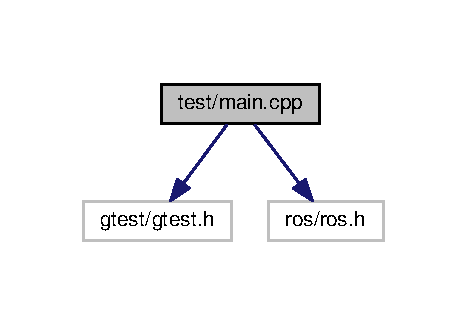
\includegraphics[width=224pt]{main_8cpp__incl}
\end{center}
\end{figure}
\subsection*{Functions}
\begin{DoxyCompactItemize}
\item 
int \hyperlink{main_8cpp_a3c04138a5bfe5d72780bb7e82a18e627}{main} (int argc, char $\ast$$\ast$argv)
\end{DoxyCompactItemize}


\subsection{Detailed Description}
Test implementation of class test. 

B\+SD 3-\/\+Clause License

\begin{DoxyCopyright}{Copyright}
(c) 2019, Naman Gupta, Umang Rastogi All rights reserved. Redistribution and use in source and binary forms, with or without modification, are permitted provided that the following conditions are met\+:
\end{DoxyCopyright}
Redistributions of source code must retain the above copyright notice, this list of conditions and the following disclaimer. Redistributions in binary form must reproduce the above copyright notice, this list of conditions and the following disclaimer in the documentation and/or other materials provided with the distribution. Neither the name of the copyright holder nor the names of its contributors may be used to endorse or promote products derived from this software without specific prior written permission. T\+H\+IS S\+O\+F\+T\+W\+A\+RE IS P\+R\+O\+V\+I\+D\+ED BY T\+HE C\+O\+P\+Y\+R\+I\+G\+HT H\+O\+L\+D\+E\+RS A\+ND C\+O\+N\+T\+R\+I\+B\+U\+T\+O\+RS \char`\"{}\+A\+S I\+S\char`\"{} A\+ND A\+NY E\+X\+P\+R\+E\+SS OR I\+M\+P\+L\+I\+ED W\+A\+R\+R\+A\+N\+T\+I\+ES, I\+N\+C\+L\+U\+D\+I\+NG, B\+UT N\+OT L\+I\+M\+I\+T\+ED TO, T\+HE I\+M\+P\+L\+I\+ED W\+A\+R\+R\+A\+N\+T\+I\+ES OF M\+E\+R\+C\+H\+A\+N\+T\+A\+B\+I\+L\+I\+TY A\+ND F\+I\+T\+N\+E\+SS F\+OR A P\+A\+R\+T\+I\+C\+U\+L\+AR P\+U\+R\+P\+O\+SE A\+RE D\+I\+S\+C\+L\+A\+I\+M\+ED. IN NO E\+V\+E\+NT S\+H\+A\+LL T\+HE C\+O\+P\+Y\+R\+I\+G\+HT H\+O\+L\+D\+ER OR C\+O\+N\+T\+R\+I\+B\+U\+T\+O\+RS BE L\+I\+A\+B\+LE F\+OR A\+NY D\+I\+R\+E\+CT, I\+N\+D\+I\+R\+E\+CT, I\+N\+C\+I\+D\+E\+N\+T\+AL, S\+P\+E\+C\+I\+AL, E\+X\+E\+M\+P\+L\+A\+RY, OR C\+O\+N\+S\+E\+Q\+U\+E\+N\+T\+I\+AL D\+A\+M\+A\+G\+ES (I\+N\+C\+L\+U\+D\+I\+NG, B\+UT N\+OT L\+I\+M\+I\+T\+ED TO, P\+R\+O\+C\+U\+R\+E\+M\+E\+NT OF S\+U\+B\+S\+T\+I\+T\+U\+TE G\+O\+O\+DS OR S\+E\+R\+V\+I\+C\+ES; L\+O\+SS OF U\+SE, D\+A\+TA, OR P\+R\+O\+F\+I\+TS; OR B\+U\+S\+I\+N\+E\+SS I\+N\+T\+E\+R\+R\+U\+P\+T\+I\+ON) H\+O\+W\+E\+V\+ER C\+A\+U\+S\+ED A\+ND ON A\+NY T\+H\+E\+O\+RY OF L\+I\+A\+B\+I\+L\+I\+TY, W\+H\+E\+T\+H\+ER IN C\+O\+N\+T\+R\+A\+CT, S\+T\+R\+I\+CT L\+I\+A\+B\+I\+L\+I\+TY, OR T\+O\+RT (I\+N\+C\+L\+U\+D\+I\+NG N\+E\+G\+L\+I\+G\+E\+N\+CE OR O\+T\+H\+E\+R\+W\+I\+SE) A\+R\+I\+S\+I\+NG IN A\+NY W\+AY O\+UT OF T\+HE U\+SE OF T\+H\+IS S\+O\+F\+T\+W\+A\+RE, E\+V\+EN IF A\+D\+V\+I\+S\+ED OF T\+HE P\+O\+S\+S\+I\+B\+I\+L\+I\+TY OF S\+U\+CH D\+A\+M\+A\+GE.

\begin{DoxyAuthor}{Author}
Naman Gupta -\/ Driver 

Umang Rastogi -\/ Navigator 
\end{DoxyAuthor}
\begin{DoxyVersion}{Version}
v1.\+0 
\end{DoxyVersion}


\subsection{Function Documentation}
\index{main.\+cpp@{main.\+cpp}!main@{main}}
\index{main@{main}!main.\+cpp@{main.\+cpp}}
\subsubsection[{\texorpdfstring{main(int argc, char $\ast$$\ast$argv)}{main(int argc, char **argv)}}]{\setlength{\rightskip}{0pt plus 5cm}int main (
\begin{DoxyParamCaption}
\item[{int}]{argc, }
\item[{char $\ast$$\ast$}]{argv}
\end{DoxyParamCaption}
)}\hypertarget{main_8cpp_a3c04138a5bfe5d72780bb7e82a18e627}{}\label{main_8cpp_a3c04138a5bfe5d72780bb7e82a18e627}

\hypertarget{object__detection__test_8cpp}{}\section{test/object\+\_\+detection\+\_\+test.cpp File Reference}
\label{object__detection__test_8cpp}\index{test/object\+\_\+detection\+\_\+test.\+cpp@{test/object\+\_\+detection\+\_\+test.\+cpp}}
{\ttfamily \#include $<$object\+\_\+detection/object\+\_\+detection.\+h$>$}\\*
{\ttfamily \#include $<$gtest/gtest.\+h$>$}\\*
{\ttfamily \#include $<$ros/ros.\+h$>$}\\*
{\ttfamily \#include \char`\"{}opencv2/opencv.\+hpp\char`\"{}}\\*
Include dependency graph for object\+\_\+detection\+\_\+test.\+cpp\+:
\nopagebreak
\begin{figure}[H]
\begin{center}
\leavevmode
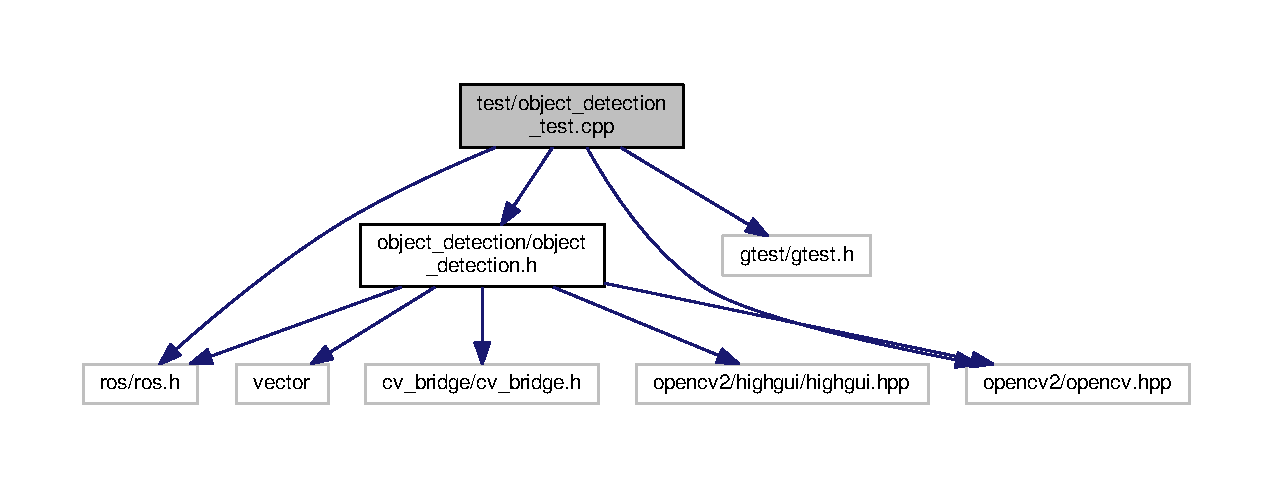
\includegraphics[width=350pt]{object__detection__test_8cpp__incl}
\end{center}
\end{figure}
\subsection*{Functions}
\begin{DoxyCompactItemize}
\item 
\hyperlink{object__detection__test_8cpp_a272dd121fe32cae77b6e2740fe43c69e}{T\+E\+ST} (Object\+Detection\+Test, object\+Not\+Detected)
\begin{DoxyCompactList}\small\item\em Test to check getters and setters. \end{DoxyCompactList}\item 
\hyperlink{object__detection__test_8cpp_a1df63b07a92a566771ca35ddc825989a}{T\+E\+ST} (Object\+Detection\+Test, object\+Detected)
\begin{DoxyCompactList}\small\item\em Test to check getters and setters. \end{DoxyCompactList}\item 
\hyperlink{object__detection__test_8cpp_a67eec44cbc8fcd243a13197dff383087}{T\+E\+ST} (Object\+Detection\+Test, set\+Boundary)
\begin{DoxyCompactList}\small\item\em Test to check setting of object boundary. \end{DoxyCompactList}\item 
\hyperlink{object__detection__test_8cpp_a235cb75479ba6461078367bf515a4f4e}{T\+E\+ST} (Object\+Detection\+Test, gauss\+Filter)
\begin{DoxyCompactList}\small\item\em Test to check gaussian filtering. \end{DoxyCompactList}\item 
\hyperlink{object__detection__test_8cpp_a683ac4af2799e9ba6b2cdf907b767680}{T\+E\+ST} (Object\+Detection\+Test, check\+Object)
\begin{DoxyCompactList}\small\item\em Test to check object detection using hsv. \end{DoxyCompactList}\end{DoxyCompactItemize}


\subsection{Function Documentation}
\index{object\+\_\+detection\+\_\+test.\+cpp@{object\+\_\+detection\+\_\+test.\+cpp}!T\+E\+ST@{T\+E\+ST}}
\index{T\+E\+ST@{T\+E\+ST}!object\+\_\+detection\+\_\+test.\+cpp@{object\+\_\+detection\+\_\+test.\+cpp}}
\subsubsection[{\texorpdfstring{T\+E\+S\+T(\+Object\+Detection\+Test, object\+Not\+Detected)}{TEST(ObjectDetectionTest, objectNotDetected)}}]{\setlength{\rightskip}{0pt plus 5cm}T\+E\+ST (
\begin{DoxyParamCaption}
\item[{Object\+Detection\+Test}]{, }
\item[{object\+Not\+Detected}]{}
\end{DoxyParamCaption}
)}\hypertarget{object__detection__test_8cpp_a272dd121fe32cae77b6e2740fe43c69e}{}\label{object__detection__test_8cpp_a272dd121fe32cae77b6e2740fe43c69e}


Test to check getters and setters. 

\index{object\+\_\+detection\+\_\+test.\+cpp@{object\+\_\+detection\+\_\+test.\+cpp}!T\+E\+ST@{T\+E\+ST}}
\index{T\+E\+ST@{T\+E\+ST}!object\+\_\+detection\+\_\+test.\+cpp@{object\+\_\+detection\+\_\+test.\+cpp}}
\subsubsection[{\texorpdfstring{T\+E\+S\+T(\+Object\+Detection\+Test, object\+Detected)}{TEST(ObjectDetectionTest, objectDetected)}}]{\setlength{\rightskip}{0pt plus 5cm}T\+E\+ST (
\begin{DoxyParamCaption}
\item[{Object\+Detection\+Test}]{, }
\item[{object\+Detected}]{}
\end{DoxyParamCaption}
)}\hypertarget{object__detection__test_8cpp_a1df63b07a92a566771ca35ddc825989a}{}\label{object__detection__test_8cpp_a1df63b07a92a566771ca35ddc825989a}


Test to check getters and setters. 

\index{object\+\_\+detection\+\_\+test.\+cpp@{object\+\_\+detection\+\_\+test.\+cpp}!T\+E\+ST@{T\+E\+ST}}
\index{T\+E\+ST@{T\+E\+ST}!object\+\_\+detection\+\_\+test.\+cpp@{object\+\_\+detection\+\_\+test.\+cpp}}
\subsubsection[{\texorpdfstring{T\+E\+S\+T(\+Object\+Detection\+Test, set\+Boundary)}{TEST(ObjectDetectionTest, setBoundary)}}]{\setlength{\rightskip}{0pt plus 5cm}T\+E\+ST (
\begin{DoxyParamCaption}
\item[{Object\+Detection\+Test}]{, }
\item[{set\+Boundary}]{}
\end{DoxyParamCaption}
)}\hypertarget{object__detection__test_8cpp_a67eec44cbc8fcd243a13197dff383087}{}\label{object__detection__test_8cpp_a67eec44cbc8fcd243a13197dff383087}


Test to check setting of object boundary. 

Define object boundary \index{object\+\_\+detection\+\_\+test.\+cpp@{object\+\_\+detection\+\_\+test.\+cpp}!T\+E\+ST@{T\+E\+ST}}
\index{T\+E\+ST@{T\+E\+ST}!object\+\_\+detection\+\_\+test.\+cpp@{object\+\_\+detection\+\_\+test.\+cpp}}
\subsubsection[{\texorpdfstring{T\+E\+S\+T(\+Object\+Detection\+Test, gauss\+Filter)}{TEST(ObjectDetectionTest, gaussFilter)}}]{\setlength{\rightskip}{0pt plus 5cm}T\+E\+ST (
\begin{DoxyParamCaption}
\item[{Object\+Detection\+Test}]{, }
\item[{gauss\+Filter}]{}
\end{DoxyParamCaption}
)}\hypertarget{object__detection__test_8cpp_a235cb75479ba6461078367bf515a4f4e}{}\label{object__detection__test_8cpp_a235cb75479ba6461078367bf515a4f4e}


Test to check gaussian filtering. 

Check if file empty or not

These two images do not hace the same size due to smoothening \index{object\+\_\+detection\+\_\+test.\+cpp@{object\+\_\+detection\+\_\+test.\+cpp}!T\+E\+ST@{T\+E\+ST}}
\index{T\+E\+ST@{T\+E\+ST}!object\+\_\+detection\+\_\+test.\+cpp@{object\+\_\+detection\+\_\+test.\+cpp}}
\subsubsection[{\texorpdfstring{T\+E\+S\+T(\+Object\+Detection\+Test, check\+Object)}{TEST(ObjectDetectionTest, checkObject)}}]{\setlength{\rightskip}{0pt plus 5cm}T\+E\+ST (
\begin{DoxyParamCaption}
\item[{Object\+Detection\+Test}]{, }
\item[{check\+Object}]{}
\end{DoxyParamCaption}
)}\hypertarget{object__detection__test_8cpp_a683ac4af2799e9ba6b2cdf907b767680}{}\label{object__detection__test_8cpp_a683ac4af2799e9ba6b2cdf907b767680}


Test to check object detection using hsv. 

Check for condition when obstacle not detected 
\hypertarget{obstacle__avoidance__test_8cpp}{}\section{test/obstacle\+\_\+avoidance\+\_\+test.cpp File Reference}
\label{obstacle__avoidance__test_8cpp}\index{test/obstacle\+\_\+avoidance\+\_\+test.\+cpp@{test/obstacle\+\_\+avoidance\+\_\+test.\+cpp}}


Class test implementation of class \hyperlink{classObstacleAvoidance}{Obstacle\+Avoidance}.  


{\ttfamily \#include $<$obstacle\+\_\+avoidance/obstacle\+\_\+avoidance.\+h$>$}\\*
{\ttfamily \#include $<$gtest/gtest.\+h$>$}\\*
{\ttfamily \#include $<$ros/ros.\+h$>$}\\*
Include dependency graph for obstacle\+\_\+avoidance\+\_\+test.\+cpp\+:\nopagebreak
\begin{figure}[H]
\begin{center}
\leavevmode
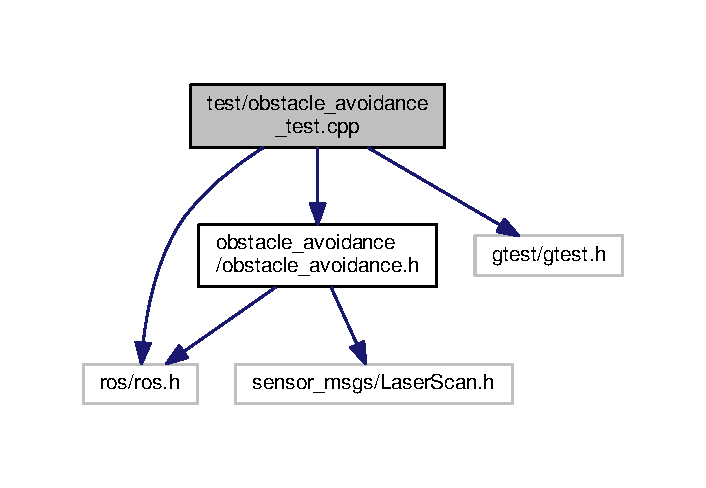
\includegraphics[width=339pt]{obstacle__avoidance__test_8cpp__incl}
\end{center}
\end{figure}
\subsection*{Functions}
\begin{DoxyCompactItemize}
\item 
\hyperlink{obstacle__avoidance__test_8cpp_ac1cd47bac47de1c96d3d8f657785c396}{T\+E\+ST} (Obstacle\+Avoidance\+Test, obstacle\+Not\+Detected)
\begin{DoxyCompactList}\small\item\em Test to check obstacle detected or not. \end{DoxyCompactList}\item 
\hyperlink{obstacle__avoidance__test_8cpp_acc0db72dbbfe6921be935ec106314d8d}{T\+E\+ST} (Obstacle\+Avoidance\+Test, obstacle\+Detected)
\begin{DoxyCompactList}\small\item\em Test to check getters and setters. \end{DoxyCompactList}\item 
\hyperlink{obstacle__avoidance__test_8cpp_ace97a9ce4db229f4a62e8dbda4848f19}{T\+E\+ST} (Obstacle\+Avoidance\+Test, check\+Obstacle)
\begin{DoxyCompactList}\small\item\em Test to check obstacle. \end{DoxyCompactList}\end{DoxyCompactItemize}


\subsection{Detailed Description}
Class test implementation of class \hyperlink{classObstacleAvoidance}{Obstacle\+Avoidance}. 

B\+SD 3-\/\+Clause License

\begin{DoxyCopyright}{Copyright}
(c) 2019, Naman Gupta, Umang Rastogi All rights reserved. Redistribution and use in source and binary forms, with or without modification, are permitted provided that the following conditions are met\+:
\end{DoxyCopyright}
Redistributions of source code must retain the above copyright notice, this list of conditions and the following disclaimer. Redistributions in binary form must reproduce the above copyright notice, this list of conditions and the following disclaimer in the documentation and/or other materials provided with the distribution. Neither the name of the copyright holder nor the names of its contributors may be used to endorse or promote products derived from this software without specific prior written permission. T\+H\+IS S\+O\+F\+T\+W\+A\+RE IS P\+R\+O\+V\+I\+D\+ED BY T\+HE C\+O\+P\+Y\+R\+I\+G\+HT H\+O\+L\+D\+E\+RS A\+ND C\+O\+N\+T\+R\+I\+B\+U\+T\+O\+RS \char`\"{}\+A\+S I\+S\char`\"{} A\+ND A\+NY E\+X\+P\+R\+E\+SS OR I\+M\+P\+L\+I\+ED W\+A\+R\+R\+A\+N\+T\+I\+ES, I\+N\+C\+L\+U\+D\+I\+NG, B\+UT N\+OT L\+I\+M\+I\+T\+ED TO, T\+HE I\+M\+P\+L\+I\+ED W\+A\+R\+R\+A\+N\+T\+I\+ES OF M\+E\+R\+C\+H\+A\+N\+T\+A\+B\+I\+L\+I\+TY A\+ND F\+I\+T\+N\+E\+SS F\+OR A P\+A\+R\+T\+I\+C\+U\+L\+AR P\+U\+R\+P\+O\+SE A\+RE D\+I\+S\+C\+L\+A\+I\+M\+ED. IN NO E\+V\+E\+NT S\+H\+A\+LL T\+HE C\+O\+P\+Y\+R\+I\+G\+HT H\+O\+L\+D\+ER OR C\+O\+N\+T\+R\+I\+B\+U\+T\+O\+RS BE L\+I\+A\+B\+LE F\+OR A\+NY D\+I\+R\+E\+CT, I\+N\+D\+I\+R\+E\+CT, I\+N\+C\+I\+D\+E\+N\+T\+AL, S\+P\+E\+C\+I\+AL, E\+X\+E\+M\+P\+L\+A\+RY, OR C\+O\+N\+S\+E\+Q\+U\+E\+N\+T\+I\+AL D\+A\+M\+A\+G\+ES (I\+N\+C\+L\+U\+D\+I\+NG, B\+UT N\+OT L\+I\+M\+I\+T\+ED TO, P\+R\+O\+C\+U\+R\+E\+M\+E\+NT OF S\+U\+B\+S\+T\+I\+T\+U\+TE G\+O\+O\+DS OR S\+E\+R\+V\+I\+C\+ES; L\+O\+SS OF U\+SE, D\+A\+TA, OR P\+R\+O\+F\+I\+TS; OR B\+U\+S\+I\+N\+E\+SS I\+N\+T\+E\+R\+R\+U\+P\+T\+I\+ON) H\+O\+W\+E\+V\+ER C\+A\+U\+S\+ED A\+ND ON A\+NY T\+H\+E\+O\+RY OF L\+I\+A\+B\+I\+L\+I\+TY, W\+H\+E\+T\+H\+ER IN C\+O\+N\+T\+R\+A\+CT, S\+T\+R\+I\+CT L\+I\+A\+B\+I\+L\+I\+TY, OR T\+O\+RT (I\+N\+C\+L\+U\+D\+I\+NG N\+E\+G\+L\+I\+G\+E\+N\+CE OR O\+T\+H\+E\+R\+W\+I\+SE) A\+R\+I\+S\+I\+NG IN A\+NY W\+AY O\+UT OF T\+HE U\+SE OF T\+H\+IS S\+O\+F\+T\+W\+A\+RE, E\+V\+EN IF A\+D\+V\+I\+S\+ED OF T\+HE P\+O\+S\+S\+I\+B\+I\+L\+I\+TY OF S\+U\+CH D\+A\+M\+A\+GE.

\begin{DoxyAuthor}{Author}
Naman Gupta -\/ Driver 

Umang Rastogi -\/ Navigator
\end{DoxyAuthor}
Test the methods of class \hyperlink{classObstacleAvoidance}{Obstacle\+Avoidance} 

\subsection{Function Documentation}
\index{obstacle\+\_\+avoidance\+\_\+test.\+cpp@{obstacle\+\_\+avoidance\+\_\+test.\+cpp}!T\+E\+ST@{T\+E\+ST}}
\index{T\+E\+ST@{T\+E\+ST}!obstacle\+\_\+avoidance\+\_\+test.\+cpp@{obstacle\+\_\+avoidance\+\_\+test.\+cpp}}
\subsubsection[{\texorpdfstring{T\+E\+S\+T(\+Obstacle\+Avoidance\+Test, obstacle\+Not\+Detected)}{TEST(ObstacleAvoidanceTest, obstacleNotDetected)}}]{\setlength{\rightskip}{0pt plus 5cm}T\+E\+ST (
\begin{DoxyParamCaption}
\item[{Obstacle\+Avoidance\+Test}]{, }
\item[{obstacle\+Not\+Detected}]{}
\end{DoxyParamCaption}
)}\hypertarget{obstacle__avoidance__test_8cpp_ac1cd47bac47de1c96d3d8f657785c396}{}\label{obstacle__avoidance__test_8cpp_ac1cd47bac47de1c96d3d8f657785c396}


Test to check obstacle detected or not. 

\index{obstacle\+\_\+avoidance\+\_\+test.\+cpp@{obstacle\+\_\+avoidance\+\_\+test.\+cpp}!T\+E\+ST@{T\+E\+ST}}
\index{T\+E\+ST@{T\+E\+ST}!obstacle\+\_\+avoidance\+\_\+test.\+cpp@{obstacle\+\_\+avoidance\+\_\+test.\+cpp}}
\subsubsection[{\texorpdfstring{T\+E\+S\+T(\+Obstacle\+Avoidance\+Test, obstacle\+Detected)}{TEST(ObstacleAvoidanceTest, obstacleDetected)}}]{\setlength{\rightskip}{0pt plus 5cm}T\+E\+ST (
\begin{DoxyParamCaption}
\item[{Obstacle\+Avoidance\+Test}]{, }
\item[{obstacle\+Detected}]{}
\end{DoxyParamCaption}
)}\hypertarget{obstacle__avoidance__test_8cpp_acc0db72dbbfe6921be935ec106314d8d}{}\label{obstacle__avoidance__test_8cpp_acc0db72dbbfe6921be935ec106314d8d}


Test to check getters and setters. 

\index{obstacle\+\_\+avoidance\+\_\+test.\+cpp@{obstacle\+\_\+avoidance\+\_\+test.\+cpp}!T\+E\+ST@{T\+E\+ST}}
\index{T\+E\+ST@{T\+E\+ST}!obstacle\+\_\+avoidance\+\_\+test.\+cpp@{obstacle\+\_\+avoidance\+\_\+test.\+cpp}}
\subsubsection[{\texorpdfstring{T\+E\+S\+T(\+Obstacle\+Avoidance\+Test, check\+Obstacle)}{TEST(ObstacleAvoidanceTest, checkObstacle)}}]{\setlength{\rightskip}{0pt plus 5cm}T\+E\+ST (
\begin{DoxyParamCaption}
\item[{Obstacle\+Avoidance\+Test}]{, }
\item[{check\+Obstacle}]{}
\end{DoxyParamCaption}
)}\hypertarget{obstacle__avoidance__test_8cpp_ace97a9ce4db229f4a62e8dbda4848f19}{}\label{obstacle__avoidance__test_8cpp_ace97a9ce4db229f4a62e8dbda4848f19}


Test to check obstacle. 

Define distance threshold for obstacles 
\hypertarget{turtlebot__test_8cpp}{}\section{test/turtlebot\+\_\+test.cpp File Reference}
\label{turtlebot__test_8cpp}\index{test/turtlebot\+\_\+test.\+cpp@{test/turtlebot\+\_\+test.\+cpp}}
{\ttfamily \#include $<$turtlebot/turtlebot.\+h$>$}\\*
{\ttfamily \#include $<$gtest/gtest.\+h$>$}\\*
{\ttfamily \#include $<$ros/ros.\+h$>$}\\*
Include dependency graph for turtlebot\+\_\+test.\+cpp\+:
\nopagebreak
\begin{figure}[H]
\begin{center}
\leavevmode
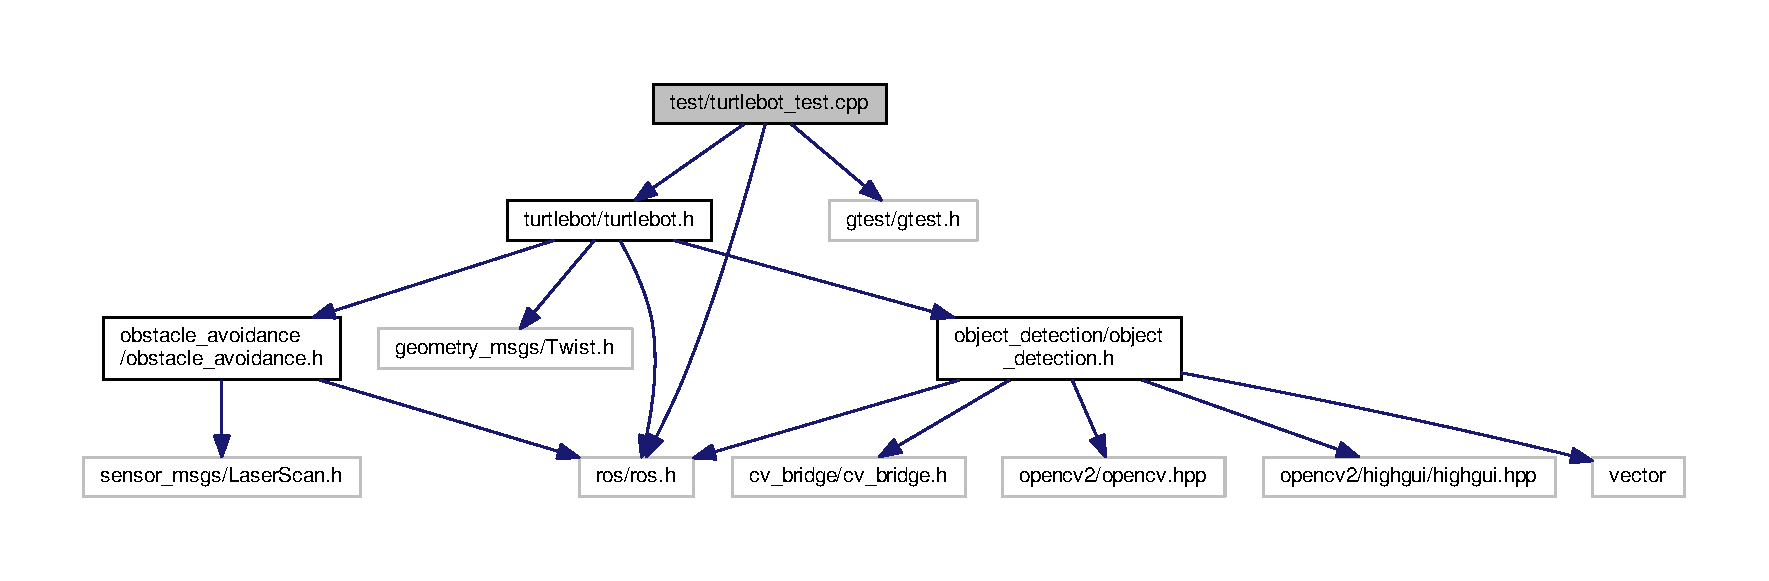
\includegraphics[width=323pt]{turtlebot__test_8cpp__incl}
\end{center}
\end{figure}
\subsection*{Functions}
\begin{DoxyCompactItemize}
\item 
\hyperlink{turtlebot__test_8cpp_a9a6ea4dc6684bb026f62cfdda7aff1f1}{T\+E\+ST} (Turtlebot\+Test, velocity\+Changed\+Test)
\begin{DoxyCompactList}\small\item\em Test to check obstacle detected or not. \end{DoxyCompactList}\item 
\hyperlink{turtlebot__test_8cpp_af6ae717c41dd4bf43eb1cc32725c0f80}{T\+E\+ST} (Turtlebot\+Test, move\+Forward\+Test)
\begin{DoxyCompactList}\small\item\em Test for move\+Forward() method  Test to check linear velocity provided to method. \end{DoxyCompactList}\item 
\hyperlink{turtlebot__test_8cpp_ab47b3f4f1f1ae5d087ed79fdd0f5b6c4}{T\+E\+ST} (Turtlebot\+Test, turn\+Test)
\begin{DoxyCompactList}\small\item\em Test for turn() method  Test to check angular velocity provided to method. \end{DoxyCompactList}\end{DoxyCompactItemize}


\subsection{Function Documentation}
\index{turtlebot\+\_\+test.\+cpp@{turtlebot\+\_\+test.\+cpp}!T\+E\+ST@{T\+E\+ST}}
\index{T\+E\+ST@{T\+E\+ST}!turtlebot\+\_\+test.\+cpp@{turtlebot\+\_\+test.\+cpp}}
\subsubsection[{\texorpdfstring{T\+E\+S\+T(\+Turtlebot\+Test, velocity\+Changed\+Test)}{TEST(TurtlebotTest, velocityChangedTest)}}]{\setlength{\rightskip}{0pt plus 5cm}T\+E\+ST (
\begin{DoxyParamCaption}
\item[{Turtlebot\+Test}]{, }
\item[{velocity\+Changed\+Test}]{}
\end{DoxyParamCaption}
)}\hypertarget{turtlebot__test_8cpp_a9a6ea4dc6684bb026f62cfdda7aff1f1}{}\label{turtlebot__test_8cpp_a9a6ea4dc6684bb026f62cfdda7aff1f1}


Test to check obstacle detected or not. 

\index{turtlebot\+\_\+test.\+cpp@{turtlebot\+\_\+test.\+cpp}!T\+E\+ST@{T\+E\+ST}}
\index{T\+E\+ST@{T\+E\+ST}!turtlebot\+\_\+test.\+cpp@{turtlebot\+\_\+test.\+cpp}}
\subsubsection[{\texorpdfstring{T\+E\+S\+T(\+Turtlebot\+Test, move\+Forward\+Test)}{TEST(TurtlebotTest, moveForwardTest)}}]{\setlength{\rightskip}{0pt plus 5cm}T\+E\+ST (
\begin{DoxyParamCaption}
\item[{Turtlebot\+Test}]{, }
\item[{move\+Forward\+Test}]{}
\end{DoxyParamCaption}
)}\hypertarget{turtlebot__test_8cpp_af6ae717c41dd4bf43eb1cc32725c0f80}{}\label{turtlebot__test_8cpp_af6ae717c41dd4bf43eb1cc32725c0f80}


Test for move\+Forward() method  Test to check linear velocity provided to method. 

\index{turtlebot\+\_\+test.\+cpp@{turtlebot\+\_\+test.\+cpp}!T\+E\+ST@{T\+E\+ST}}
\index{T\+E\+ST@{T\+E\+ST}!turtlebot\+\_\+test.\+cpp@{turtlebot\+\_\+test.\+cpp}}
\subsubsection[{\texorpdfstring{T\+E\+S\+T(\+Turtlebot\+Test, turn\+Test)}{TEST(TurtlebotTest, turnTest)}}]{\setlength{\rightskip}{0pt plus 5cm}T\+E\+ST (
\begin{DoxyParamCaption}
\item[{Turtlebot\+Test}]{, }
\item[{turn\+Test}]{}
\end{DoxyParamCaption}
)}\hypertarget{turtlebot__test_8cpp_ab47b3f4f1f1ae5d087ed79fdd0f5b6c4}{}\label{turtlebot__test_8cpp_ab47b3f4f1f1ae5d087ed79fdd0f5b6c4}


Test for turn() method  Test to check angular velocity provided to method. 


%--- End generated contents ---

% Index
\backmatter
\newpage
\phantomsection
\clearemptydoublepage
\addcontentsline{toc}{chapter}{Index}
\printindex

\end{document}
